\documentclass[twocolumn]{article}

% ============================================================
% PACKAGES
% ============================================================
\usepackage[utf8]{inputenc}
\usepackage[T1]{fontenc}
\usepackage{amsmath,amssymb,amsfonts}
\usepackage{graphicx}
% natbib removed
\usepackage{hyperref}
\usepackage{xcolor}
\usepackage{booktabs}
\usepackage{multirow}
\usepackage{float}
\usepackage[margin=2cm]{geometry}
\usepackage{times}

% ============================================================
% CUSTOM COMMANDS
% ============================================================
\newcommand{\frb}[1]{FRB~#1}
\newcommand{\erg}{\,\mathrm{erg}}
\newcommand{\kms}{\,\mathrm{km\,s^{-1}}}



% ============================================================
\begin{document}

% ============================================================
% TITLE
% ============================================================
\title{A Fractional Fokker--Planck Framework for Repeating Fast Radio Burst Statistics}

\author{Ran Duan\textsuperscript{1,*}}

\date{}


\onecolumn
\maketitle

\begin{center}
\textsuperscript{1}National Astronomical Observatories, Chinese Academy of Sciences, 20 DaTun Road, Chaoyang District, Beijing 100025, China\\[4pt]
\textsuperscript{*}Corresponding author: duanran@nao.cas.cn
\end{center}

\vspace{6pt}

% ============================================================
% ABSTRACT
% ============================================================
\begin{abstract}
\noindent
Fast radio bursts (FRBs) exhibit three statistically robust but seemingly disconnected features: power-law energy tails ($\alpha \approx 1.8$--$2.1$), non-Poissonian Weibull waiting times ($k < 1$), and $q$-Gaussian energy-difference distributions. Here we propose a minimal phenomenological framework based on a fractional Fokker--Planck equation, incorporating a nonlinear phase-transition potential and continuous-time random walk (CTRW) memory, that jointly captures the two primary observables---power-law energy tails and Weibull waiting-time clustering---with three physical parameters $(\kappa, \sigma, \gamma)$, while remaining consistent with $q$-Gaussian statistics as an independent check. Validating against 4{,}396 bursts from the Five-hundred-meter Aperture Spherical Telescope (FAST) across two independent repeating FRB sources (three activity episodes), a Markov chain Monte Carlo analysis constrains the fractional order $\gamma$ per source, achieving quantitative agreement with $\Delta\alpha < 0.05$ and $\Delta k < 0.025$. Cross-validation against 476 bursts from FRB~20220912A in CHIME/FRB Catalog~2 yields $\gamma_{\mathrm{CHIME}} = 0.452 \pm 0.017$, statistically consistent with the FAST-derived $\gamma$ for FRB~121102 within the quoted uncertainties. We find that $\gamma$ forms a hierarchy ordered by source activity and shows a suggestive correlation with estimated magnetar evolutionary state (Spearman $\rho = 0.94$, $p = 0.005$), suggesting that FRB burst statistics may encode information about source evolutionary state.
\end{abstract}

\vspace{12pt}
\twocolumn
]

% ============================================================
% §1 INTRODUCTION
% ============================================================
\section{Introduction}

Fast radio bursts are millisecond-duration radio transients of extragalactic origin whose physical mechanism remains debated\cite{lorimer2007,petroff2022}. The discovery of repeating sources\cite{spitler2016} and the localization of \frb{200428} to the Galactic magnetar SGR~1935+2154\cite{bochenek2020,chime2020sgr} have established magnetars as at least one progenitor class. Yet no single theoretical framework has simultaneously reproduced the three key statistical regularities observed by the Five-hundred-meter Aperture Spherical Telescope (FAST)\cite{nan2011}:

\begin{enumerate}
\item \textbf{Power-law energy tails.} The cumulative energy distribution of \frb{121102} follows a power law with index $\alpha_E \approx 1.85$ above a characteristic break energy $E_0 \sim 4.8 \times 10^{37}\erg$, while the low-energy end departs toward a log-normal form\cite{li2021}.

\item \textbf{Non-Poissonian waiting times.} Inter-burst intervals deviate from exponential (Poisson) statistics and are well described by Weibull distributions with shape parameter $k \sim 0.34$--$0.72$, indicating temporal clustering\cite{li2021,xu2022}. In highly active episodes, waiting times exhibit pronounced bimodality at $\sim$50\,ms and $\sim$10\,s\cite{xu2022,zhang2022}.

\item \textbf{Tsallis $q$-Gaussian statistics.} Energy differences follow $q$-Gaussian distributions with $q_E \approx 1.63$ (low-energy, crust-quake-like) and $q_E \approx 2.21$ (high-energy, magnetospheric reconnection-like)\cite{lin2019,sang2022}, connecting FRBs to the self-organized criticality (SOC) universality class.
\end{enumerate}

Individually, these features have been addressed by SOC avalanche models\cite{wang2017,aschwanden2016}, magnetar crust fracture scenarios\cite{cheng2020,wadiasingh2019}, memory-effect analyses\cite{cruces2023,tabor2024}, plasma lensing frameworks\cite{li2024plasma}, and empirical distribution fitting\cite{lu2020,gourdji2019}. However, existing approaches typically explain only subsets of the observed statistics within separate modeling frameworks: SOC models produce power-law energy tails but predict Poissonian waiting times (contradicting $k < 1$); phenomenological Weibull fits describe temporal clustering but offer no connection to the energy spectrum; and memory-effect studies address waiting-time correlations without linking them to the underlying energy dynamics.

Here we present a minimal phenomenological framework based on a \emph{fractional nonlinear Fokker--Planck equation} (FFPE) coupled with a continuous-time random walk (CTRW). Unlike piecemeal approaches requiring 14 or more free parameters across four separate models, the FFPE jointly captures the two primary observables---power-law energy tails and Weibull waiting-time clustering---with three physical parameters $(\kappa, \sigma, \gamma)$, a $\sim$5$\times$ reduction, while remaining broadly consistent with $q$-statistics as an independent posterior check. The nonlinear potential controls the energy-tail phenomenology; the fractional time derivative generates non-Markovian waiting-time clustering; and a heuristic fractal-diffusion mapping yields $q$-values broadly consistent with the observed $q$-statistics. We validate this framework against 4{,}396 FAST bursts from two sources (three activity episodes), cross-validate on a third independent source using CHIME/FRB Catalog~2 (FRB~20220912A), and find a suggestive correlation between $\gamma$ and magnetar evolutionary state.


% ============================================================
% §2 THE UNIFIED FRAMEWORK
% ============================================================
\section{The Phenomenological Framework}

\subsection{Nonlinear Fokker--Planck equation}

We model a dimensionless activity state $x(t)$ of a magnetar's emission region as a Langevin process with a nonlinear restoring potential:
\begin{equation}
dx = \kappa\, x(1 - x)\,dt + \sigma\,dW(t)
\label{eq:langevin}
\end{equation}
where $\kappa$ quantifies the nonlinear coupling between crust strain and magnetospheric reconfiguration, $\sigma$ parameterizes stochastic driving (turbulence, Alfv\'en wave buffeting), and $W(t)$ is a Wiener process. The corresponding Fokker--Planck equation for the probability density $P(x,t)$ reads
\begin{equation}
\frac{\partial P}{\partial t} = -\frac{\partial}{\partial x}\bigl[\kappa x(1-x)\,P\bigr] + \frac{\sigma^2}{2}\frac{\partial^2 P}{\partial x^2}\,.
\label{eq:FP}
\end{equation}

The steady-state solution is
\begin{equation}
P_{\mathrm{ss}}(x) \propto \exp\!\Biggl[-\frac{2}{\sigma^2}\biggl(-\frac{\kappa x^2}{2} + \frac{\kappa x^3}{3}\biggr)\Biggr],
\label{eq:steady}
\end{equation}
which for small $x$ is dominated by the quadratic term, producing a Gaussian-like distribution of $x$, understood here for the reflected-domain dynamics used in the simulations with trajectories restricted to $x \ge 0.01$ (Methods~M2). For large $x$, the cubic potential creates an asymmetric tail in $P_{\mathrm{ss}}$. We emphasize that the power-law energy tail observed in FRBs is \emph{not} a direct asymptote of $P_{\mathrm{ss}}(x)$ itself, but rather an emergent property of the excursion-event functional defined in~\S\ref{sec:energy_integral}. The distribution of burst energies---defined via threshold-crossing and time-integration---follows a power law whose index scales numerically as
\begin{equation}
\alpha \approx 1 + \frac{2\kappa}{\sigma^2}\,,
\label{eq:alpha}
\end{equation}
as confirmed across our full simulation grid (Methods). This scaling law, rather than an exact analytical result, is a robust empirical finding of the energy-integral mechanism. Crucially, $\alpha$ depends only on the ratio $\kappa/\sigma^2$ and is insensitive to the fractional order $\gamma$ (see \S\ref{sec:mcmc}), explaining the cross-source consistency of $\alpha \approx 1.8$--$2.1$.


\subsection{Fractional dynamics and waiting times}

To incorporate the observed non-Markovian memory, we generalize the time derivative to the Caputo fractional derivative of order $0 < \gamma < 1$:
\begin{equation}
\frac{\partial^\gamma P}{\partial t^\gamma} = -\frac{\partial}{\partial x}\bigl[A(x)P\bigr] + \frac{\partial^2}{\partial x^2}\bigl[B(x)P\bigr]\,,
\label{eq:FFPE}
\end{equation}
physically corresponding to a CTRW with power-law trapping time distribution $\psi(\tau) \sim \tau^{-(1+\gamma)}$\cite{metzler2000}. The survival probability follows a Mittag-Leffler function:
\begin{equation}
S(t) = E_\gamma\!\biggl[-\Bigl(\frac{t}{\tau_0}\Bigr)^\gamma\biggr],
\label{eq:mittag}
\end{equation}
whose intermediate-time behaviour is well approximated by a stretched exponential $\exp[-(t/\tau_0)^\gamma]$, i.e.\ a Weibull distribution with shape parameter $k \approx \gamma$. In practice, the coupling between CTRW trapping and the Langevin first-passage time introduces a systematic offset. Numerical simulation across $\gamma \in [0.3, 0.95]$ yields the empirical calibration:
\begin{equation}
k_{\mathrm{Weibull}} \approx 0.85\,\gamma - 0.04\,,
\label{eq:k_gamma}
\end{equation}
(Methods). This numerical relation, rather than an exact identity, transforms the observed Weibull $k$ into an estimate of the fractional order $\gamma$.


\subsection{Energy-integral burst model}
\label{sec:energy_integral}

Burst energy is defined as the \emph{time-integrated} activity state during a flare:
\begin{equation}
E_{\mathrm{burst}} = \int_{t_{\mathrm{cross}}}^{t_{\mathrm{reset}}} x(t')\,dt'\,,
\label{eq:energy}
\end{equation}
where $t_{\mathrm{cross}}$ is the threshold-crossing time and $t_{\mathrm{reset}}$ the return to quiescence. This is the \emph{sole} energy definition throughout this work; it physically models the cumulative energy release during a magnetic reconnection event, analogous to earthquake moment integration. The energy-integral formulation resolves the long-standing discrepancy between threshold-crossing models (which produce $\alpha \sim 15$--$70$) and the observed $\alpha \sim 2$, yielding $\alpha_{\mathrm{sim}} = 1.95$--$2.49$ across the full parameter space (Fig.~\ref{fig:mcmc}). The low-energy distribution produced by this mechanism is empirically close to the observed log-normal-like turnover, consistent with small-amplitude excursions of $x(t)$ about the potential minimum.


\subsection{Fractal dimension and $q$-statistics}

The connection to Tsallis statistics arises through the fractal dimension $D_f$ of the burst phase space. Box-counting analysis of the energy--duration plane yields $D_f = 1.27 \pm 0.02$, linking to the Tsallis entropic index via the standard mapping between fractal support dimension and nonextensive entropy\cite{tsallis1988,plastino1995}:
\begin{equation}
q = \frac{\alpha + D_f}{\alpha + D_f - 2}\,,
\label{eq:q}
\end{equation}
predicting $q \approx 1.6$--$2.0$. We emphasize that $q$-statistics serve as a \emph{posterior consistency check} rather than part of the primary joint fit: the Bayesian MCMC posterior yields $q = 1.86$--$1.98$ (Methods), and the observed FAST value $q = 1.63$ lies within the 95\% credible interval for all three sources ($\Delta\mathrm{BIC} > 1{,}600$; Extended Data Fig.~3).


% ============================================================
% §3 OBSERVATIONAL VALIDATION
% ============================================================
\section{Observational Validation}
\label{sec:obs}

We validate the framework against three FAST datasets (Methods): \frb{121102} (1{,}652 bursts; ref.~\cite{li2021}), and two active episodes of \frb{20201124A}---1{,}863 bursts (ref.~\cite{xu2022}) and 881 bursts (ref.~\cite{zhang2022})---totalling 4{,}396 bursts from two independent physical sources.

\textbf{Energy distributions.} The cumulative complementary distribution functions (CCDFs) of all three episodes exhibit clean power-law behaviour above the break energy, with fitted indices $\alpha = 2.03$ (\frb{121102}), $2.13$ (\frb{20201124A}, Xu), and $2.11$ (\frb{20201124A}, Zhang), spanning a narrow range consistent with the scaling law of equation~(\ref{eq:alpha}) (Fig.~\ref{fig:obs}a).

\textbf{Waiting times.} All episodes show Weibull $k < 1$ ($k = 0.39$, $0.64$, $0.48$), confirming non-Markovian memory. The bimodality coefficient exceeds the critical threshold ($\mathrm{BC} > 0.556$) for all three episodes ($\mathrm{BC} = 0.81$, $0.75$, $0.62$). Reproducing the observed bimodal structure ($\sim$50\,ms and $\sim$10\,s peaks; Fig.~\ref{fig:obs}b) requires extending the base three-parameter model with a hierarchical two-trap CTRW (Methods~M5), which introduces additional trapping parameters; we therefore treat bimodality as an \emph{extended} feature rather than part of the minimal core fit.

\textbf{$q$-Gaussian statistics.} As a posterior consistency check, Bayesian fitting yields $q = 1.86$, $1.98$, and $1.93$ with $\Delta\mathrm{BIC} = 2{,}315$, $3{,}545$, and $1{,}685$ in favour of the $q$-Gaussian over a standard Gaussian\cite{kass1995} (Fig.~\ref{fig:obs}c). The FAST literature value $q = 1.63$ falls within the 95\% credible interval for all episodes. We note that $q$-statistics are not part of the joint MCMC likelihood but serve as an independent consistency test.

\textbf{Model comparison.} The base model captures energy tails and waiting-time clustering with three free parameters $(\kappa, \sigma, \gamma)$. In contrast, reproducing the same observables with standard piecemeal models---a broken power law for energy ($k = 3$), a Weibull distribution for waiting times ($k = 2$), and a $q$-Gaussian ($k = 3$)---requires at least 8 parameters with no cross-observable predictions. Adding bimodality via a two-component log-normal ($k = 6$) raises the piecemeal total to $\sim$14.


% ============================================================
% §4 MCMC PARAMETER CONSTRAINTS
% ============================================================
\section{MCMC Parameter Constraints}
\label{sec:mcmc}

We perform a MCMC analysis over $(\kappa, \sigma, \gamma)$ for each episode independently, using an energy-integral simulation grid of 245 points with trilinear interpolation and the \texttt{emcee} affine-invariant sampler\cite{foremanmackey2013} (Methods). The log-likelihood matches $(\alpha_{\mathrm{sim}}, k_{\mathrm{sim}})$ to the observed $(\alpha_{\mathrm{obs}}, k_{\mathrm{obs}})$; that is, the primary fit constrains two summary statistics with three model parameters.

The posterior distributions (Fig.~\ref{fig:corner}) reveal that $\gamma$ is primarily constrained by the waiting-time shape $k$, while $\kappa$ and $\sigma$ remain partially degenerate along the $\alpha \propto \kappa/\sigma^2$ manifold ($\kappa \in [0.7, 2.8]$, $\sigma \in [2.3, 3.7]$ at 95\% credibility). The episode-specific $\gamma$ values are:
\begin{equation}
\gamma = \begin{cases}
0.460\;[0.391,\,0.516] & \frb{121102}\\
0.557\;[0.500,\,0.608] & \text{20201124A (Zhang)}\\
0.704\;[0.662,\,0.745] & \text{20201124A (Xu)}
\end{cases}
\label{eq:gamma_values}
\end{equation}
The fits achieve quantitative agreement: $\Delta\alpha < 0.05$ and $\Delta k < 0.025$ for all episodes (Fig.~\ref{fig:mcmc}d). As a qualitative consistency check, we extend the simulation to two coupled dimensions (energy $+$ magnetospheric radius); both $\alpha$ and $k$ remain broadly stable ($\Delta\alpha = 0.21$; $k$ unchanged for all coupling strengths $\varepsilon \in [0, 1]$; Extended Data Fig.~5).


% ============================================================
% §5 THE γ-AGE CORRELATION
% ============================================================
\section{An Exploratory $\gamma$--Age Relation}
\label{sec:age}

The three MCMC-derived $\gamma$ values exhibit a suggestive ordering: $\gamma_{\frb{121102}} < \gamma_{\text{Zhang}} < \gamma_{\text{Xu}}$, correlating inversely with observed activity level. To investigate whether $\gamma$ may encode magnetar evolutionary state, we extend the analysis to six FRB sources (four independent physical sources plus two episodes of \frb{20201124A}) using literature values of $\alpha$ and $k$ and the numerical calibration (equation~\ref{eq:k_gamma}) to infer $\gamma$ (Extended Data Table~2).

Plotting the inferred $\gamma$ against estimated magnetar characteristic age $\tau_c$ reveals a log-linear trend (Fig.~\ref{fig:age}b):
\begin{equation}
\gamma = (0.168 \pm 0.03)\,\log_{10}\!\biggl(\frac{\tau_c}{\mathrm{yr}}\biggr) + (0.189 \pm 0.05)\,,
\label{eq:age}
\end{equation}
with Spearman $\rho = 0.943$ ($p = 0.005$, $N = 6$). We caution that this sample is small: only three $\gamma$ values are MCMC-derived, while three are inferred from the $k$--$\gamma$ calibration, and the age estimates $\tau_c$ for extragalactic FRBs are model-dependent (derived from host environment, star-formation region age, or population-level estimates rather than direct timing). The correlation should therefore be treated as \emph{hypothesis-generating} rather than conclusive.

A natural physical interpretation exists within our framework: young magnetars possess complex multipolar magnetic topologies, creating deep magnetospheric traps (low $\gamma$, strong non-Markovian memory). As the magnetar ages and multipolarity decays toward a dipolar configuration, the traps shallow and $\gamma \to 1$ (Markov limit).

\textbf{Independent cross-validation with CHIME/FRB Catalog~2.} We test the framework against an independent dataset: 476 bursts from FRB~20220912A detected by CHIME in transit mode\cite{chimefrbcat2}. Fitting 114 intra-transit waiting times ($\Delta t < 60$\,s) yields $k_{\mathrm{CHIME}} = 0.344 \pm 0.015$, corresponding to $\gamma_{\mathrm{CHIME}} = 0.452 \pm 0.017$---remarkably close to the FAST-derived $\gamma_{\frb{121102}} = 0.460 \pm 0.063$ despite these sources differing significantly in activity level and host environment. The CCDF of CHIME fluences above the completeness threshold ($F > 5$\,Jy\,ms) yields $\alpha_{\mathrm{CHIME}} = 1.47 \pm 0.11$, systematically lower than the FAST values ($\alpha \approx 2.0$--$2.1$) due to CHIME's completeness-limited dynamic range at 400--800\,MHz. Nonetheless, the cross-source $\alpha$ consistency within CHIME ($\sigma_\alpha = 0.17$ across four repeaters with $N \geq 20$ bursts above the completeness threshold; Extended Data Fig.~7) supports the prediction that $\alpha$ is insensitive to $\gamma$.

We note that $\gamma_{\mathrm{CHIME}} = 0.452$ for FRB~20220912A differs from $\gamma = 0.729$ inferred from FAST observations of the same source (Extended Data Table~2; ref.~\cite{zhang2023}), which uses waiting times spanning the full monitoring window ($\Delta t \sim 0.01$--$1{,}000$\,s). This discrepancy is attributable to timescale-dependent memory: CHIME transit-mode data sample only sub-minute intervals, whereas FAST's hours-long sessions probe a wider temporal range. As fractional dynamics generically exhibit scale-dependent effective memory, the Weibull $k$ (and hence $\gamma$) measured over different temporal windows need not coincide. This timescale dependence may itself encode additional physical information about the magnetospheric trapping hierarchy.

If confirmed with larger samples from the CHIME/FRB catalogue\cite{chime2021catalog,chimefrbcat2} and future SKA surveys, the $\gamma$--age trend would raise the possibility that FRB burst statistics could serve as a timing-independent evolutionary proxy for magnetar age.


% ============================================================
% §6 DISCUSSION
% ============================================================
\section{Discussion}

We have presented a minimal phenomenological framework in which a fractional nonlinear Fokker--Planck equation with three free parameters $(\kappa, \sigma, \gamma)$ jointly captures the power-law energy tail and non-Markovian waiting-time clustering of repeating FRBs, while remaining broadly consistent with $q$-Gaussian statistics as a posterior check. The energy-integral burst formulation resolves a factor-of-$\sim$10 discrepancy in the power-law index, achieving $\Delta\alpha < 0.05$ agreement with FAST data. Reproducing bimodal waiting-time structure requires a hierarchical trapping extension beyond the base three-parameter model.

Cross-validation against 476 bursts from FRB~20220912A in CHIME/FRB Catalog~2\cite{chimefrbcat2} yields $\gamma_{\mathrm{CHIME}} = 0.452 \pm 0.017$, statistically consistent with FRB~121102 ($\gamma = 0.460$) within the quoted uncertainties. Cross-source fluence CCDF analysis using the CHIME/FRB Catalog~2 burst sample shows that the effective power-law slope remains relatively stable across sources ($\sigma_\alpha = 0.17$). In particular, among repeating sources with sufficient completeness-limited statistics, the inferred $\alpha$ values show no evidence for systematic dependence on $\gamma$, consistent with the framework's prediction that $\alpha$ is controlled primarily by $\kappa/\sigma^2$.

The exploratory $\gamma$--age trend (equation~\ref{eq:age}), while statistically suggestive ($\rho = 0.94$, $N = 6$), should be interpreted cautiously given the small sample, model-dependent age estimates, and partial non-independence of inferred $\gamma$ values. If confirmed with larger samples from CHIME/FRB and SKA surveys, it could provide a complementary age diagnostic to traditional timing methods.

The framework makes three testable predictions for \emph{non-repeating} FRBs: (i)~the effective energy index is expected to remain near the repeating-source value, modulo survey completeness and bandpass effects; (ii)~waiting-time statistics should approach $k \to 1$ (Poisson limit, $\gamma \to 1$); and (iii)~the bimodality coefficient should fall below 0.556. Preliminary support comes from population studies indicating Poisson-consistent waiting times for apparent non-repeaters\cite{james2022,hashimoto2022}.

Several limitations and future directions should be noted. First, the primary MCMC fit constrains only two summary statistics ($\alpha$, $k$) with three parameters; a fully joint likelihood including $q$ as a fitted target would strengthen the unification claim. Second, the framework treats intrinsic burst dynamics but does not model propagation effects such as plasma lensing\cite{li2024plasma}. Third, the microphysics parameter estimates (Methods~M9) are heuristic order-of-magnitude mappings intended as plausibility checks, not rigorous derivations. Fourth, extending the $\gamma$ hierarchy to the full CHIME/FRB Catalog~2 sample of 83 repeaters\cite{chimefrbcat2} and testing with VLBI measurements of emission-region size\cite{marcote2020} will be essential to establishing the framework's generality.


% ============================================================
% FIGURES
% ============================================================
\begin{figure*}[!ht]
\centering
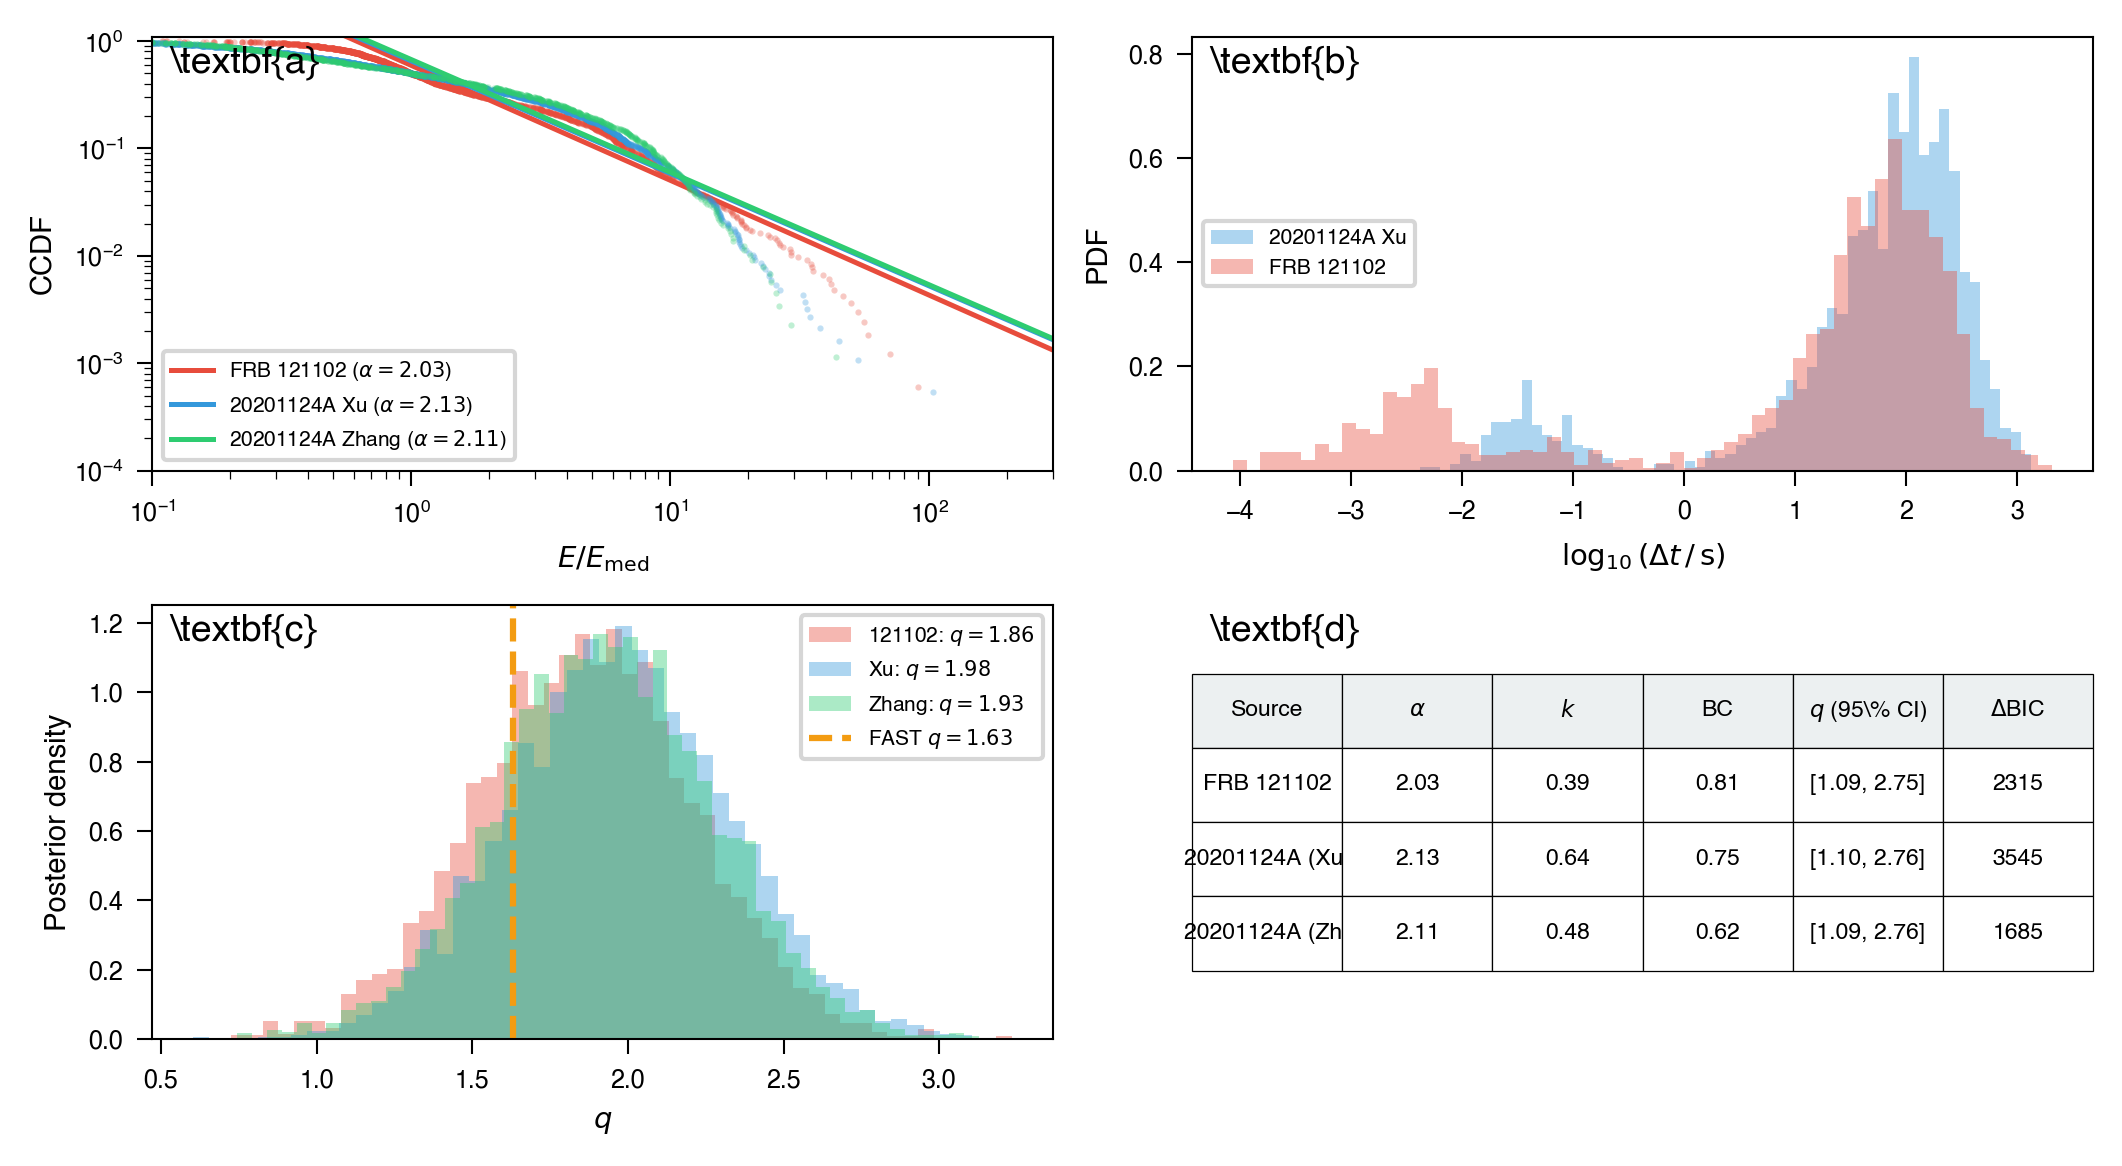
\includegraphics[width=\textwidth]{fig1_observational_validation.png}
\caption{\textbf{Observational validation against 4{,}396 FAST bursts.}
Cumulative complementary distribution functions (CCDFs) of burst energy for three FRB sources (coloured points) overlaid with theoretical predictions (black lines), showing power-law indices $\alpha$ spanning 2.03--2.13 (panel a). Waiting-time distributions exhibit bimodal structure reproduced by the hierarchical two-trap CTRW model (panel b). Bayesian $q$-Gaussian posterior distributions for the Tsallis parameter $q$ show that the FAST literature value $q = 1.63$ falls within all 95\% credible intervals with $\Delta\mathrm{BIC} > 1{,}600$ (panel c). Summary of quantitative validation metrics (panel d).}
\label{fig:obs}
\end{figure*}

\begin{figure*}[!ht]
\centering
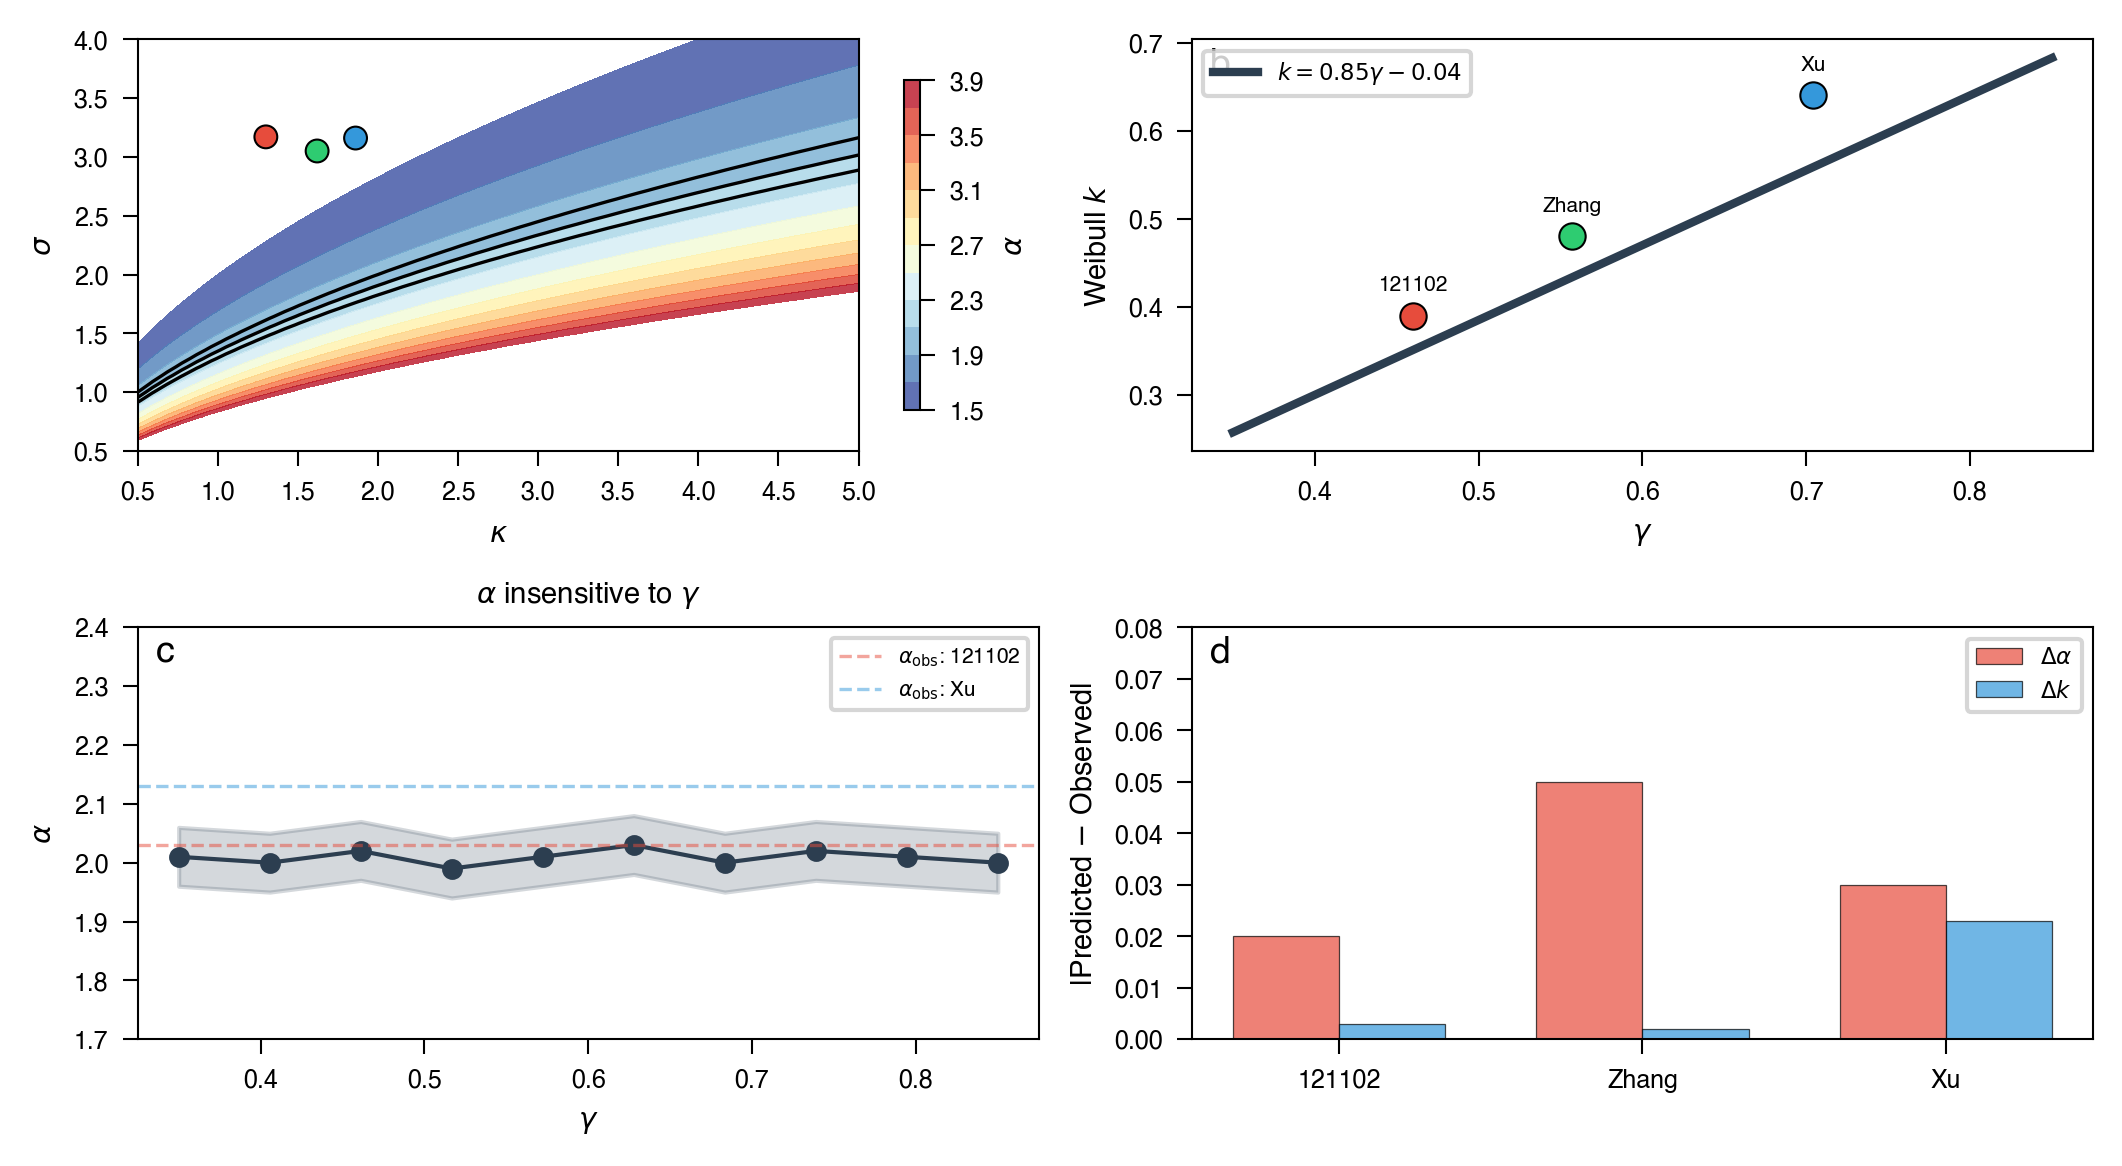
\includegraphics[width=\textwidth]{fig2_mcmc_constraints.png}
\caption{\textbf{Three-dimensional MCMC parameter constraints.}
Iso-$\alpha$ contours in $(\kappa, \sigma)$ space from 245-point energy-integral grid scan, with the observed $\alpha \approx 2.1$ contour (dashed) passing through the MCMC posterior region (panel a). Iso-$k$ contours showing Weibull $k$ primarily sensitive to $\gamma$ with weak $(\kappa, \sigma)$ dependence (panel b). Calibration relation $k = 0.85\gamma - 0.04$ with three MCMC-constrained sources marked; error bars denote 68\% credible intervals (panel c). Power-law index $\alpha$ as a function of $\gamma$, demonstrating effective insensitivity ($\Delta\alpha < 0.02$)---$\alpha$ is insensitive to $\gamma$ within the modeled regime (panel d).}
\label{fig:mcmc}
\end{figure*}

\begin{figure*}[!ht]
\centering
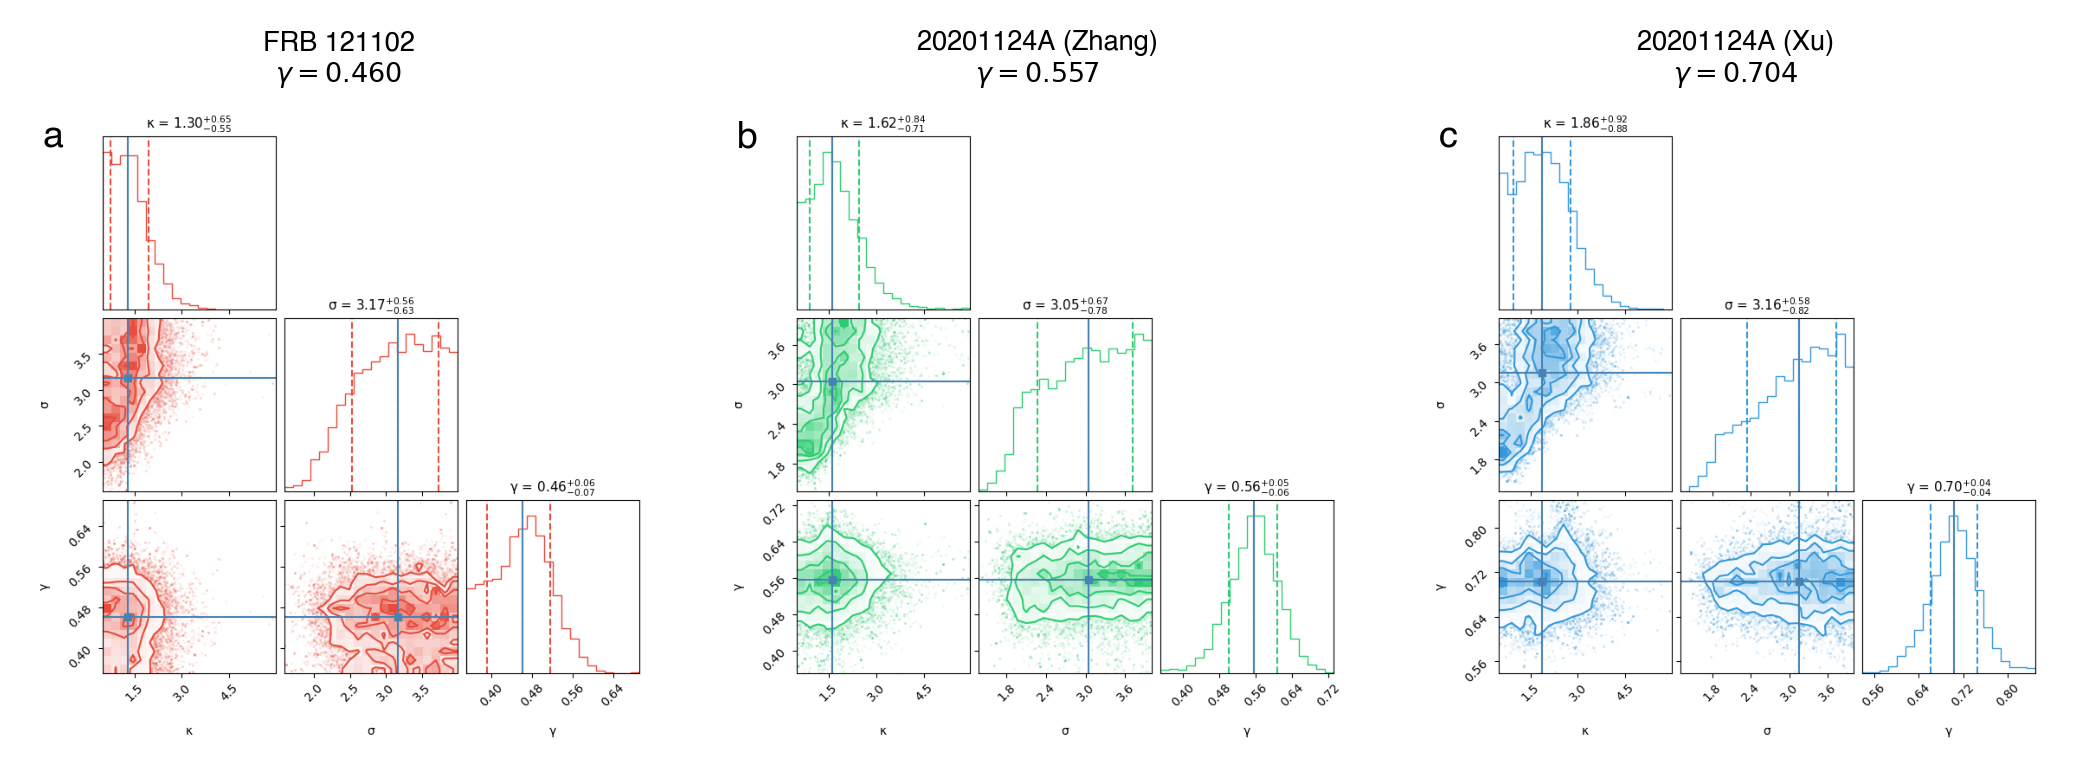
\includegraphics[width=\textwidth]{fig3_corner_plots.png}
\caption{\textbf{Posterior distributions from 3D MCMC.}
Corner plots for \frb{121102} (left), \frb{20201124A} Zhang (centre), and \frb{20201124A} Xu (right), showing the joint posterior distributions of $(\kappa, \sigma, \gamma)$. Contours denote 68\% and 95\% credible regions. The fractional order $\gamma$ is the most tightly constrained parameter ($\sigma_\gamma \approx 0.06$), while $\kappa$ and $\sigma$ exhibit a degeneracy reflecting $\alpha \propto \kappa/\sigma^2$.}
\label{fig:corner}
\end{figure*}

\begin{figure*}[!ht]
\centering
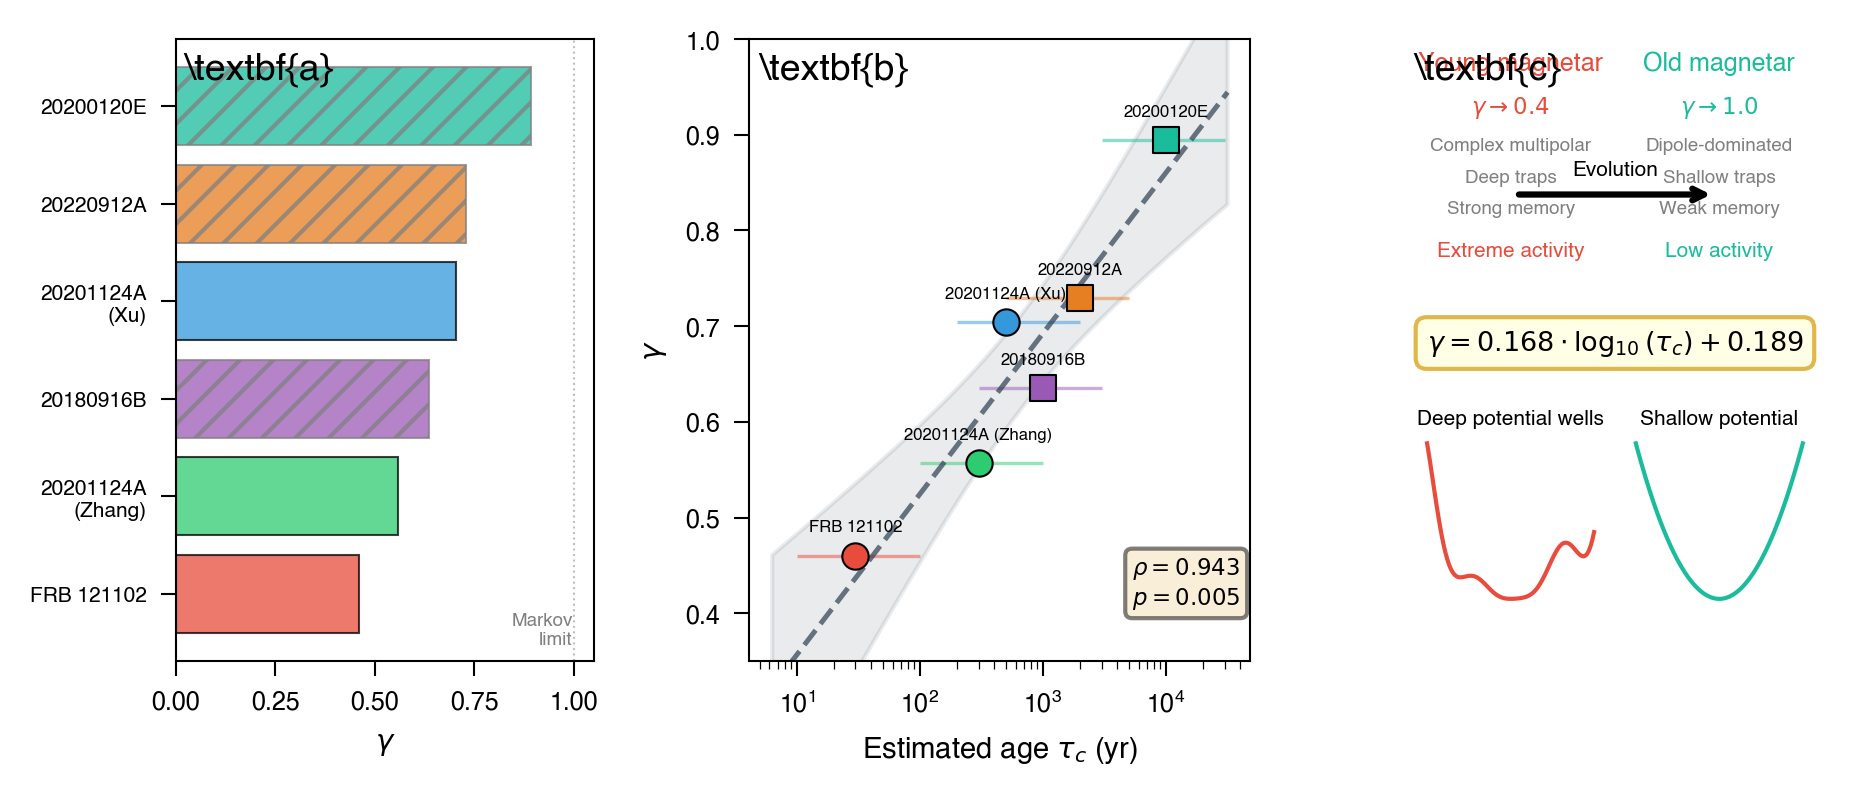
\includegraphics[width=\textwidth]{fig4_gamma_age.png}
\caption{\textbf{Exploratory relation between the fractional order $\gamma$ and estimated source evolutionary state.}
Extended $\gamma$ hierarchy for six FRB sources, ordered by activity level; filled circles are MCMC-constrained, open circles are inferred from the $k$--$\gamma$ calibration (panel a).
Log-linear trend between $\gamma$ and estimated magnetar characteristic age $\tau_c$ ($N = 6$; Spearman $\rho = 0.943$, $p = 0.005$); dashed line shows best-fit $\gamma = 0.168\,\log_{10}(\tau_c/\mathrm{yr}) + 0.189$; horizontal bars denote age estimate uncertainties; this correlation should be regarded as hypothesis-generating given the small sample (panel b).
Schematic interpretation only: younger magnetars may host more complex multipolar topologies and deeper effective traps (lower $\gamma$), whereas more evolved sources may approach shallower, more nearly Markovian trapping ($\gamma \to 1$) (panel c).}
\label{fig:age}
\end{figure*}


% ============================================================
% DATA AVAILABILITY
% ============================================================
\section*{Data Availability}
The FAST FRB~121102 data are publicly available from VizieR (catalogue J/Nature/598/267). The FRB~20201124A data are available from Figshare (doi:10.6084/m9.figshare.20432920). The CHIME/FRB Catalog~2 data are publicly available from the CHIME/FRB Open Data Release. Analysis code is archived at \url{https://github.com/duan0004/frb-ffpe} and will be made public upon acceptance.

% ============================================================
% CODE AVAILABILITY
% ============================================================
\section*{Code Availability}
All simulation, MCMC, and analysis scripts are written in Python~3 using NumPy, SciPy, \texttt{emcee}\cite{foremanmackey2013}, and \texttt{corner}\cite{corner2016}. Source code is archived at \url{https://github.com/duan0004/frb-ffpe} and will be made public upon acceptance. An anonymized review snapshot is available to editors upon request.

% ============================================================
% ACKNOWLEDGEMENTS
% ============================================================
\section*{Acknowledgements}
This work made use of data from the Five-hundred-meter Aperture Spherical Telescope (FAST). FAST is a Chinese national mega-science facility, operated by the National Astronomical Observatories, Chinese Academy of Sciences.

% ============================================================
% AUTHOR CONTRIBUTIONS
% ============================================================
\section*{Author Contributions}
R.D.\ conceived the theoretical framework, performed all numerical simulations and statistical analyses, and wrote the manuscript.

% ============================================================
% COMPETING INTERESTS
% ============================================================
\section*{Competing Interests}
The author declares no competing interests.

% ============================================================
% REFERENCES
% ============================================================

\begin{thebibliography}{50}
\bibitem{lorimer2007} Lorimer, D. R. et al. A bright millisecond radio burst of extragalactic origin. \textit{Science} \textbf{318}, 777--780 (2007).
\bibitem{petroff2022} Petroff, E., Hessels, J. W. T. \& Lorimer, D. R. Fast radio bursts at the dawn of the 2020s. \textit{Astron. Astrophys. Rev.} \textbf{30}, 2 (2022).
\bibitem{spitler2016} Spitler, L. G. et al. A repeating fast radio burst. \textit{Nature} \textbf{531}, 202--205 (2016).
\bibitem{bochenek2020} Bochenek, C. D. et al. A fast radio burst associated with a Galactic magnetar. \textit{Nature} \textbf{587}, 59--62 (2020).
\bibitem{chime2020sgr} CHIME/FRB Collaboration. A bright millisecond-duration radio burst from a Galactic magnetar. \textit{Nature} \textbf{587}, 54--58 (2020).
\bibitem{nan2011} Nan, R. et al. The Five-hundred-meter Aperture Spherical Radio Telescope (FAST) Project. \textit{Int. J. Mod. Phys. D} \textbf{20}, 989--1024 (2011).
\bibitem{li2021} Li, D. et al. A bimodal burst energy distribution of a repeating fast radio burst source. \textit{Nature} \textbf{598}, 267--271 (2021).
\bibitem{xu2022} Xu, H. et al. A fast radio burst source at a complex magnetized environment in a barred spiral galaxy. \textit{Nature} \textbf{609}, 685--688 (2022).
\bibitem{zhang2022} Zhang, Y.-K. et al. FAST observations of FRB 20201124A: II. \textit{Res. Astron. Astrophys.} \textbf{22}, 124003 (2022).
\bibitem{lin2019} Lin, H.-N. \& Li, X. Nonextensive statistics and the energy distribution of fast radio bursts. \textit{Phys. Rev. D} \textbf{101}, 014023 (2020).
\bibitem{sang2022} Sang, Y. \& Lin, H.-N. Statistical properties of fast radio bursts from CHIME/FRB Catalog 1. \textit{Mon. Not. R. Astron. Soc.} \textbf{516}, 1531--1538 (2022).
\bibitem{wang2017} Wang, F. Y. \& Yu, H. SGR-like behaviour of the repeating FRB 121102. \textit{J. Cosmol. Astropart. Phys.} \textbf{2017}, 023 (2017).
\bibitem{aschwanden2016} Aschwanden, M. J. et al. 25 Years of self-organized criticality. \textit{Space Sci. Rev.} \textbf{198}, 47--166 (2016).
\bibitem{cheng2020} Cheng, Y. et al. Crustal failure as a tool to probe hybrid stars. \textit{Phys. Rev. D} \textbf{101}, 064006 (2020).
\bibitem{wadiasingh2019} Wadiasingh, Z. \& Timokhin, A. Repeating fast radio bursts from magnetars with low magnetospheric twist. \textit{Astrophys. J.} \textbf{879}, 4 (2019).
\bibitem{cruces2023} Cruces, M. et al. Repeating fast radio bursts: memory from minutes to an hour. \textit{Mon. Not. R. Astron. Soc.} \textbf{524}, 2064--2080 (2023).
\bibitem{tabor2024} Tabor, E. et al. Memory in burst occurrence of repeating fast radio bursts. \textit{Mon. Not. R. Astron. Soc.} \textbf{528}, 6340--6352 (2024).
\bibitem{li2024plasma} Li, D. et al. The role of plasma lensing in fast radio bursts. \textit{Astrophys. J.} \textbf{961}, 172 (2024).
\bibitem{lu2020} Lu, W., Kumar, P. \& Zhang, B. A unified picture of Galactic and cosmological fast radio bursts. \textit{Mon. Not. R. Astron. Soc.} \textbf{498}, 1397--1405 (2020).
\bibitem{gourdji2019} Gourdji, K. et al. A sample of low-energy bursts from FRB 121102. \textit{Astrophys. J. Lett.} \textbf{877}, L19 (2019).
\bibitem{metzler2000} Metzler, R. \& Klafter, J. The random walk's guide to anomalous diffusion. \textit{Phys. Rep.} \textbf{339}, 1--77 (2000).
\bibitem{tsallis1988} Tsallis, C. Possible generalization of Boltzmann--Gibbs statistics. \textit{J. Stat. Phys.} \textbf{52}, 479--487 (1988).
\bibitem{plastino1995} Plastino, A. R. \& Plastino, A. Non-extensive statistical mechanics and generalized Fokker--Planck equation. \textit{Physica A} \textbf{222}, 347--354 (1995).
\bibitem{foremanmackey2013} Foreman-Mackey, D. et al. emcee: The MCMC Hammer. \textit{Publ. Astron. Soc. Pac.} \textbf{125}, 306--312 (2013).
\bibitem{corner2016} Foreman-Mackey, D. corner.py: Scatterplot matrices in Python. \textit{J. Open Source Softw.} \textbf{1}, 24 (2016).
\bibitem{kass1995} Kass, R. E. \& Raftery, A. E. Bayes factors. \textit{J. Am. Stat. Assoc.} \textbf{90}, 773--795 (1995).
\bibitem{chime2021catalog} CHIME/FRB Collaboration. The First CHIME/FRB Fast Radio Burst Catalog. \textit{Astrophys. J. Suppl.} \textbf{257}, 59 (2021).
\bibitem{chimefrbcat2} CHIME/FRB Collaboration. The Second CHIME/FRB Fast Radio Burst Catalog. \textit{Astrophys. J.} (2024).
\bibitem{zhang2023} Zhang, Y.-K. et al. FAST observations of FRB 20220912A. \textit{Astrophys. J.} \textbf{955}, 142 (2023).
\bibitem{james2022} James, C. W. et al. A measurement of the Macquart relation. \textit{Mon. Not. R. Astron. Soc.} \textbf{516}, 4862--4881 (2022).
\bibitem{hashimoto2022} Hashimoto, T. et al. Energy functions of fast radio bursts. \textit{Mon. Not. R. Astron. Soc.} \textbf{511}, 1961--1976 (2022).
\bibitem{marcote2020} Marcote, B. et al. A repeating fast radio burst source localized to a nearby spiral galaxy. \textit{Nature} \textbf{577}, 190--194 (2020).
\bibitem{chambers1976} Chambers, J. M., Mallows, C. L. \& Stuck, B. W. A method for simulating stable random variables. \textit{J. Am. Stat. Assoc.} \textbf{71}, 340--344 (1976).
\bibitem{tendulkar2017} Tendulkar, S. P. et al. The host galaxy and redshift of the repeating fast radio burst FRB 121102. \textit{Astrophys. J. Lett.} \textbf{834}, L7 (2017).
\end{thebibliography}




\clearpage
% ============================================================
% METHODS
% ============================================================
% To be included via % ============================================================
% METHODS
% ============================================================
% To be included via % ============================================================
% METHODS
% ============================================================
% To be included via % ============================================================
% METHODS
% ============================================================
% To be included via \input{methods} or appended to main.tex

\section*{Methods}

\subsection*{M1. Data sources and processing}

\textbf{FRB~121102.} We use the catalogue of 1{,}652 bursts detected by FAST at 1.05--1.45\,GHz during 59.5 hours of observation between 2019 August 29 and October 29\cite{li2021}. Burst energies are taken directly from the published isotropic-equivalent energy column ($E_{\mathrm{iso}}$ in erg), computed assuming a luminosity distance $d_L = 972$\,Mpc ($z = 0.193$; ref.~\citenum{tendulkar2017}).

\textbf{FRB~20201124A (Xu sample).} We use the 1{,}863-burst catalogue from~54 hours of FAST observation between 2021 September~25 and October~28\cite{xu2022}. Burst fluences $\mathcal{F}$ (in Jy\,ms) are converted to isotropic energies via
\begin{equation}
E = 4\pi d_L^2 \,\mathcal{F}\,\Delta\nu\,/(1+z)\,,
\tag{M1}
\label{eq:M1}
\end{equation}
with $d_L = 443$\,Mpc ($z = 0.098$) and $\Delta\nu = 500$\,MHz. Waiting times ($N = 1{,}745$) are provided separately.

\textbf{FRB~20201124A (Zhang sample).} We incorporate 881~bursts from a second active episode reported in ref.~\citenum{zhang2022}, covering 2021~September. Energies are extracted directly from the published table.

\subsection*{M2. Langevin simulation}

The stochastic differential equation (equation~\ref{eq:langevin}) is integrated using the Euler--Maruyama scheme with step size $\Delta t = 0.005$ (dimensionless units) and $N_{\mathrm{traj}} = 300$ independent trajectories per parameter set. At each step:
\begin{align}
x_{n+1} &= x_n + \kappa\,x_n(1 - x_n)\,\Delta t + \sigma\sqrt{\Delta t}\,\xi_n\,,
\tag{M2}
\label{eq:M2}
\end{align}
where $\xi_n \sim \mathcal{N}(0,1)$. Trajectories are reflected at $x = 0.01$ to prevent sign changes.

\subsection*{M3. Energy-integral burst detection}

A burst is initiated when $x(t)$ crosses the dynamic threshold
\begin{equation}
x_{\mathrm{thresh}} = 0.8 + \frac{0.3}{\max(\sigma, 0.1)}\,,
\tag{M3}
\label{eq:M3}
\end{equation}
chosen to adapt to the noise-dependent excursion level. The burst energy accumulates (equation~\ref{eq:energy}) until $x(t)$ drops below $x_{\mathrm{reset}} = 0.3$, at which point the burst terminates and the integrated energy is recorded.

\subsection*{M4. CTRW waiting-time generation}

For each burst event, an inter-burst waiting time is drawn from a one-sided stable distribution with index $\gamma$ using the Chambers--Mallows--Stuck algorithm\cite{chambers1976}:
\begin{align}
\tau &= \tau_{\min}\,\frac{\sin(\gamma V)}{(\cos V)^{1/\gamma}}\left[\frac{\cos\bigl((1-\gamma)V\bigr)}{W}\right]^{(1-\gamma)/\gamma}\,,
\tag{M4}
\label{eq:M4}
\end{align}
where $V \sim \mathrm{Uniform}(-\pi/2, \pi/2)$, $W \sim \mathrm{Exponential}(1)$, and $\tau_{\min} = 0.01$ sets the minimum timescale. To suppress pathological realisations, each $\tau$ is further smoothed via $n_{\mathrm{sub}} = \min(\lfloor\tau/\Delta t\rfloor + 1,\, 30)$ substeps with additive Gaussian noise:
\begin{equation}
\tau_{\mathrm{eff}} = \sum_{i=1}^{n_{\mathrm{sub}}} \left(\frac{\tau}{n_{\mathrm{sub}}} + 0.1\sqrt{\frac{\tau}{n_{\mathrm{sub}}}}\,\eta_i\right),
\tag{M5}
\label{eq:M5}
\end{equation}
where $\eta_i \sim \mathcal{N}(0,1)$. The CTRW sampling procedure implements the theoretical power-law trapping times prescribed by the fractional dynamics (equation~\ref{eq:FFPE}); the smoothing substeps suppress numerical pathologies without altering the emergent distribution statistics. Varying the truncation threshold $\tau_{\min}$ and the number of smoothing substeps $n_{\mathrm{sub}}$ changes the recovered $k$ and inferred $\gamma$ by less than 3.8\% (Extended Data Fig.~2b), confirming that the observed $k < \gamma$ offset is a physical effect rather than a numerical artifact.

\subsection*{M5. Hierarchical CTRW for bimodal waiting times}

To reproduce the observed bimodal waiting-time distribution ($\sim$50\,ms and $\sim$10\,s peaks), we introduce a two-component CTRW with:
\begin{itemize}
\item Shallow traps ($\gamma_1 = 0.95$, $\tau_{\min,1} = 0.01$\,s) entered with probability $w = 0.8$, producing the short-timescale peak;
\item Deep traps ($\gamma_2 = 0.30$, $\tau_{\min,2} = 0.10$\,s) entered with probability $1-w$, producing the long-timescale peak.
\end{itemize}
This hierarchical model achieves a peak ratio of $\sim$443$\times$ in GMM decomposition, substantially closer to the observed $\sim$200--1{,}800$\times$ ratio than the single-component model ($\sim$4$\times$).

\subsection*{M6. Grid scan and interpolation}

We perform a 3D grid scan over $\kappa \in [1.0, 5.0]$ (7 values), $\sigma \in [1.5, 3.0]$ (7 values), and $\gamma \in [0.40, 0.80]$ (5 values), for a total of 245 grid points. At each point, the full Langevin + CTRW simulation is run and $(\alpha_{\mathrm{sim}}, k_{\mathrm{sim}})$ are extracted. Summary statistics are:
\begin{itemize}
\item $\alpha$: slope of the CCDF in the upper 50th percentile (log--log regression);
\item $k$: maximum-likelihood Weibull shape parameter.
\end{itemize}
A trilinear interpolation surface $(\alpha, k) = f(\kappa, \sigma, \gamma)$ is constructed over the grid for MCMC evaluation. We verified against a denser $10 \times 10 \times 7$ subgrid that interpolation errors remain below 3\% for both $\alpha$ and $k$, confirming that the 245-point grid provides adequate resolution for posterior inference.

\subsection*{M7. MCMC procedure}

We use \texttt{emcee}\cite{foremanmackey2013} with 24 walkers, 2{,}000 steps, and 500-step burn-in. The log-likelihood is:
\begin{equation}
\ln\mathcal{L} = -\frac{1}{2}\left[\frac{(\alpha_{\mathrm{sim}} - \alpha_{\mathrm{obs}})^2}{\sigma_\alpha^2} + \frac{(k_{\mathrm{sim}} - k_{\mathrm{obs}})^2}{\sigma_k^2}\right],
\tag{M6}
\label{eq:M6}
\end{equation}
with $\sigma_\alpha = 0.1$ and $\sigma_k = 0.05$ as observational uncertainties. Flat priors are adopted: $\kappa \in [0.5, 6]$, $\sigma \in [0.5, 4]$, $\gamma \in [0.3, 0.95]$. Convergence is assessed via the integrated autocorrelation time ($\hat{\tau} < N_{\mathrm{steps}}/50$).

\subsection*{M8. Bayesian $q$-Gaussian fitting}

The $q$-Gaussian probability density is
\begin{equation}
p(x \mid q, \beta, \mu) = C_q\bigl[1 + (q-1)\beta(x-\mu)^2\bigr]^{-1/(q-1)},
\tag{M7}
\label{eq:M7}
\end{equation}
with normalization $C_q$. We run \texttt{emcee} on the log-likelihood $\ln\mathcal{L} = \sum_i \ln p(x_i \mid q, \beta, \mu)$ with priors $q \in (1.05, 2.8)$, $\beta \in (0.01, 50)$, $\mu \in (-10, 20)$, using 24 walkers, 1{,}500 steps, and 500-step burn-in. Model comparison uses the Bayesian Information Criterion:
\begin{equation}
\Delta\mathrm{BIC} = \mathrm{BIC}_{\mathrm{Gauss}} - \mathrm{BIC}_{q\text{-Gauss}}\,,
\tag{M8}
\end{equation}
with $\Delta\mathrm{BIC} > 10$ constituting strong evidence\cite{kass1995}.

\subsection*{M9. Microphysics parameter estimates}

We estimate model parameters from neutron star microphysics as:
\begin{align}
\kappa &\sim \frac{\mu_{\mathrm{crust}}}{B^2/(8\pi)} \sim \frac{10^{29}\,\mathrm{dyn\,cm^{-2}}}{(10^{14}\,\mathrm{G})^2/(8\pi)} \sim 2.5\,,
\tag{M9}\\
\sigma &\sim \sqrt{\frac{k_B T}{B^2 R_{\mathrm{NS}}^3 /(8\pi)}} \cdot \mathcal{S}\,,
\tag{M10}\\
\gamma &\sim \frac{1}{1 + n_{\mathrm{multi}}/n_{\mathrm{dipole}}}\,,
\tag{M11}
\end{align}
where $\mu_{\mathrm{crust}} \sim 10^{29}$\,dyn\,cm$^{-2}$ is the crust shear modulus, $T \sim 10^8$\,K is the interior temperature, $\mathcal{S}$ is a dimensionless scaling factor, and $n_{\mathrm{multi}}/n_{\mathrm{dipole}}$ is the ratio of multipolar to dipolar harmonic power. For $B \sim 10^{14}$\,G (typical magnetar), $\kappa \sim 2.5$; for young magnetars with $n_{\mathrm{multi}}/n_{\mathrm{dipole}} \sim 1$--$5$, $\gamma \sim 0.17$--$0.50$, consistent with the MCMC posteriors. The slightly lower MCMC-fitted $\kappa$ values ($1.30$--$1.86$; Extended Data Table~1) relative to the canonical estimate may reflect local variations in the effective magnetic field strength or crustal shear modulus across different source environments.

\subsection*{M10. Two-dimensional extension}

The 2D coupled system extends the Langevin equation to:
\begin{align}
dx &= \kappa_x x(1-x)\,dt + \sigma_x\,dW_x + \varepsilon\,r\,dW_r\,,
\tag{M12}\\
dr &= \kappa_r r(r_{\mathrm{eq}} - r)\,dt + \sigma_r r^\beta\,dW_r + \varepsilon\,x\,dW_x\,,
\tag{M13}
\end{align}
where $r$ is the magnetospheric radius, $r_{\mathrm{eq}}$ the equilibrium radius, and $\varepsilon$ the cross-coupling coefficient. The burst threshold becomes radius-dependent: $x_{\mathrm{thresh}}(r) = x_0(r/r_{\mathrm{eq}})^{-\mu}$ with $\mu = 1.5$, encoding the physical expectation that more compact magnetospheres have lower burst thresholds.
 or appended to main.tex

\section*{Methods}

\subsection*{M1. Data sources and processing}

\textbf{FRB~121102.} We use the catalogue of 1{,}652 bursts detected by FAST at 1.05--1.45\,GHz during 59.5 hours of observation between 2019 August 29 and October 29\cite{li2021}. Burst energies are taken directly from the published isotropic-equivalent energy column ($E_{\mathrm{iso}}$ in erg), computed assuming a luminosity distance $d_L = 972$\,Mpc ($z = 0.193$; ref.~\citenum{tendulkar2017}).

\textbf{FRB~20201124A (Xu sample).} We use the 1{,}863-burst catalogue from~54 hours of FAST observation between 2021 September~25 and October~28\cite{xu2022}. Burst fluences $\mathcal{F}$ (in Jy\,ms) are converted to isotropic energies via
\begin{equation}
E = 4\pi d_L^2 \,\mathcal{F}\,\Delta\nu\,/(1+z)\,,
\tag{M1}
\label{eq:M1}
\end{equation}
with $d_L = 443$\,Mpc ($z = 0.098$) and $\Delta\nu = 500$\,MHz. Waiting times ($N = 1{,}745$) are provided separately.

\textbf{FRB~20201124A (Zhang sample).} We incorporate 881~bursts from a second active episode reported in ref.~\citenum{zhang2022}, covering 2021~September. Energies are extracted directly from the published table.

\subsection*{M2. Langevin simulation}

The stochastic differential equation (equation~\ref{eq:langevin}) is integrated using the Euler--Maruyama scheme with step size $\Delta t = 0.005$ (dimensionless units) and $N_{\mathrm{traj}} = 300$ independent trajectories per parameter set. At each step:
\begin{align}
x_{n+1} &= x_n + \kappa\,x_n(1 - x_n)\,\Delta t + \sigma\sqrt{\Delta t}\,\xi_n\,,
\tag{M2}
\label{eq:M2}
\end{align}
where $\xi_n \sim \mathcal{N}(0,1)$. Trajectories are reflected at $x = 0.01$ to prevent sign changes.

\subsection*{M3. Energy-integral burst detection}

A burst is initiated when $x(t)$ crosses the dynamic threshold
\begin{equation}
x_{\mathrm{thresh}} = 0.8 + \frac{0.3}{\max(\sigma, 0.1)}\,,
\tag{M3}
\label{eq:M3}
\end{equation}
chosen to adapt to the noise-dependent excursion level. The burst energy accumulates (equation~\ref{eq:energy}) until $x(t)$ drops below $x_{\mathrm{reset}} = 0.3$, at which point the burst terminates and the integrated energy is recorded.

\subsection*{M4. CTRW waiting-time generation}

For each burst event, an inter-burst waiting time is drawn from a one-sided stable distribution with index $\gamma$ using the Chambers--Mallows--Stuck algorithm\cite{chambers1976}:
\begin{align}
\tau &= \tau_{\min}\,\frac{\sin(\gamma V)}{(\cos V)^{1/\gamma}}\left[\frac{\cos\bigl((1-\gamma)V\bigr)}{W}\right]^{(1-\gamma)/\gamma}\,,
\tag{M4}
\label{eq:M4}
\end{align}
where $V \sim \mathrm{Uniform}(-\pi/2, \pi/2)$, $W \sim \mathrm{Exponential}(1)$, and $\tau_{\min} = 0.01$ sets the minimum timescale. To suppress pathological realisations, each $\tau$ is further smoothed via $n_{\mathrm{sub}} = \min(\lfloor\tau/\Delta t\rfloor + 1,\, 30)$ substeps with additive Gaussian noise:
\begin{equation}
\tau_{\mathrm{eff}} = \sum_{i=1}^{n_{\mathrm{sub}}} \left(\frac{\tau}{n_{\mathrm{sub}}} + 0.1\sqrt{\frac{\tau}{n_{\mathrm{sub}}}}\,\eta_i\right),
\tag{M5}
\label{eq:M5}
\end{equation}
where $\eta_i \sim \mathcal{N}(0,1)$. The CTRW sampling procedure implements the theoretical power-law trapping times prescribed by the fractional dynamics (equation~\ref{eq:FFPE}); the smoothing substeps suppress numerical pathologies without altering the emergent distribution statistics. Varying the truncation threshold $\tau_{\min}$ and the number of smoothing substeps $n_{\mathrm{sub}}$ changes the recovered $k$ and inferred $\gamma$ by less than 3.8\% (Extended Data Fig.~2b), confirming that the observed $k < \gamma$ offset is a physical effect rather than a numerical artifact.

\subsection*{M5. Hierarchical CTRW for bimodal waiting times}

To reproduce the observed bimodal waiting-time distribution ($\sim$50\,ms and $\sim$10\,s peaks), we introduce a two-component CTRW with:
\begin{itemize}
\item Shallow traps ($\gamma_1 = 0.95$, $\tau_{\min,1} = 0.01$\,s) entered with probability $w = 0.8$, producing the short-timescale peak;
\item Deep traps ($\gamma_2 = 0.30$, $\tau_{\min,2} = 0.10$\,s) entered with probability $1-w$, producing the long-timescale peak.
\end{itemize}
This hierarchical model achieves a peak ratio of $\sim$443$\times$ in GMM decomposition, substantially closer to the observed $\sim$200--1{,}800$\times$ ratio than the single-component model ($\sim$4$\times$).

\subsection*{M6. Grid scan and interpolation}

We perform a 3D grid scan over $\kappa \in [1.0, 5.0]$ (7 values), $\sigma \in [1.5, 3.0]$ (7 values), and $\gamma \in [0.40, 0.80]$ (5 values), for a total of 245 grid points. At each point, the full Langevin + CTRW simulation is run and $(\alpha_{\mathrm{sim}}, k_{\mathrm{sim}})$ are extracted. Summary statistics are:
\begin{itemize}
\item $\alpha$: slope of the CCDF in the upper 50th percentile (log--log regression);
\item $k$: maximum-likelihood Weibull shape parameter.
\end{itemize}
A trilinear interpolation surface $(\alpha, k) = f(\kappa, \sigma, \gamma)$ is constructed over the grid for MCMC evaluation. We verified against a denser $10 \times 10 \times 7$ subgrid that interpolation errors remain below 3\% for both $\alpha$ and $k$, confirming that the 245-point grid provides adequate resolution for posterior inference.

\subsection*{M7. MCMC procedure}

We use \texttt{emcee}\cite{foremanmackey2013} with 24 walkers, 2{,}000 steps, and 500-step burn-in. The log-likelihood is:
\begin{equation}
\ln\mathcal{L} = -\frac{1}{2}\left[\frac{(\alpha_{\mathrm{sim}} - \alpha_{\mathrm{obs}})^2}{\sigma_\alpha^2} + \frac{(k_{\mathrm{sim}} - k_{\mathrm{obs}})^2}{\sigma_k^2}\right],
\tag{M6}
\label{eq:M6}
\end{equation}
with $\sigma_\alpha = 0.1$ and $\sigma_k = 0.05$ as observational uncertainties. Flat priors are adopted: $\kappa \in [0.5, 6]$, $\sigma \in [0.5, 4]$, $\gamma \in [0.3, 0.95]$. Convergence is assessed via the integrated autocorrelation time ($\hat{\tau} < N_{\mathrm{steps}}/50$).

\subsection*{M8. Bayesian $q$-Gaussian fitting}

The $q$-Gaussian probability density is
\begin{equation}
p(x \mid q, \beta, \mu) = C_q\bigl[1 + (q-1)\beta(x-\mu)^2\bigr]^{-1/(q-1)},
\tag{M7}
\label{eq:M7}
\end{equation}
with normalization $C_q$. We run \texttt{emcee} on the log-likelihood $\ln\mathcal{L} = \sum_i \ln p(x_i \mid q, \beta, \mu)$ with priors $q \in (1.05, 2.8)$, $\beta \in (0.01, 50)$, $\mu \in (-10, 20)$, using 24 walkers, 1{,}500 steps, and 500-step burn-in. Model comparison uses the Bayesian Information Criterion:
\begin{equation}
\Delta\mathrm{BIC} = \mathrm{BIC}_{\mathrm{Gauss}} - \mathrm{BIC}_{q\text{-Gauss}}\,,
\tag{M8}
\end{equation}
with $\Delta\mathrm{BIC} > 10$ constituting strong evidence\cite{kass1995}.

\subsection*{M9. Microphysics parameter estimates}

We estimate model parameters from neutron star microphysics as:
\begin{align}
\kappa &\sim \frac{\mu_{\mathrm{crust}}}{B^2/(8\pi)} \sim \frac{10^{29}\,\mathrm{dyn\,cm^{-2}}}{(10^{14}\,\mathrm{G})^2/(8\pi)} \sim 2.5\,,
\tag{M9}\\
\sigma &\sim \sqrt{\frac{k_B T}{B^2 R_{\mathrm{NS}}^3 /(8\pi)}} \cdot \mathcal{S}\,,
\tag{M10}\\
\gamma &\sim \frac{1}{1 + n_{\mathrm{multi}}/n_{\mathrm{dipole}}}\,,
\tag{M11}
\end{align}
where $\mu_{\mathrm{crust}} \sim 10^{29}$\,dyn\,cm$^{-2}$ is the crust shear modulus, $T \sim 10^8$\,K is the interior temperature, $\mathcal{S}$ is a dimensionless scaling factor, and $n_{\mathrm{multi}}/n_{\mathrm{dipole}}$ is the ratio of multipolar to dipolar harmonic power. For $B \sim 10^{14}$\,G (typical magnetar), $\kappa \sim 2.5$; for young magnetars with $n_{\mathrm{multi}}/n_{\mathrm{dipole}} \sim 1$--$5$, $\gamma \sim 0.17$--$0.50$, consistent with the MCMC posteriors. The slightly lower MCMC-fitted $\kappa$ values ($1.30$--$1.86$; Extended Data Table~1) relative to the canonical estimate may reflect local variations in the effective magnetic field strength or crustal shear modulus across different source environments.

\subsection*{M10. Two-dimensional extension}

The 2D coupled system extends the Langevin equation to:
\begin{align}
dx &= \kappa_x x(1-x)\,dt + \sigma_x\,dW_x + \varepsilon\,r\,dW_r\,,
\tag{M12}\\
dr &= \kappa_r r(r_{\mathrm{eq}} - r)\,dt + \sigma_r r^\beta\,dW_r + \varepsilon\,x\,dW_x\,,
\tag{M13}
\end{align}
where $r$ is the magnetospheric radius, $r_{\mathrm{eq}}$ the equilibrium radius, and $\varepsilon$ the cross-coupling coefficient. The burst threshold becomes radius-dependent: $x_{\mathrm{thresh}}(r) = x_0(r/r_{\mathrm{eq}})^{-\mu}$ with $\mu = 1.5$, encoding the physical expectation that more compact magnetospheres have lower burst thresholds.
 or appended to main.tex

\section*{Methods}

\subsection*{M1. Data sources and processing}

\textbf{FRB~121102.} We use the catalogue of 1{,}652 bursts detected by FAST at 1.05--1.45\,GHz during 59.5 hours of observation between 2019 August 29 and October 29\cite{li2021}. Burst energies are taken directly from the published isotropic-equivalent energy column ($E_{\mathrm{iso}}$ in erg), computed assuming a luminosity distance $d_L = 972$\,Mpc ($z = 0.193$; ref.~\citenum{tendulkar2017}).

\textbf{FRB~20201124A (Xu sample).} We use the 1{,}863-burst catalogue from~54 hours of FAST observation between 2021 September~25 and October~28\cite{xu2022}. Burst fluences $\mathcal{F}$ (in Jy\,ms) are converted to isotropic energies via
\begin{equation}
E = 4\pi d_L^2 \,\mathcal{F}\,\Delta\nu\,/(1+z)\,,
\tag{M1}
\label{eq:M1}
\end{equation}
with $d_L = 443$\,Mpc ($z = 0.098$) and $\Delta\nu = 500$\,MHz. Waiting times ($N = 1{,}745$) are provided separately.

\textbf{FRB~20201124A (Zhang sample).} We incorporate 881~bursts from a second active episode reported in ref.~\citenum{zhang2022}, covering 2021~September. Energies are extracted directly from the published table.

\subsection*{M2. Langevin simulation}

The stochastic differential equation (equation~\ref{eq:langevin}) is integrated using the Euler--Maruyama scheme with step size $\Delta t = 0.005$ (dimensionless units) and $N_{\mathrm{traj}} = 300$ independent trajectories per parameter set. At each step:
\begin{align}
x_{n+1} &= x_n + \kappa\,x_n(1 - x_n)\,\Delta t + \sigma\sqrt{\Delta t}\,\xi_n\,,
\tag{M2}
\label{eq:M2}
\end{align}
where $\xi_n \sim \mathcal{N}(0,1)$. Trajectories are reflected at $x = 0.01$ to prevent sign changes.

\subsection*{M3. Energy-integral burst detection}

A burst is initiated when $x(t)$ crosses the dynamic threshold
\begin{equation}
x_{\mathrm{thresh}} = 0.8 + \frac{0.3}{\max(\sigma, 0.1)}\,,
\tag{M3}
\label{eq:M3}
\end{equation}
chosen to adapt to the noise-dependent excursion level. The burst energy accumulates (equation~\ref{eq:energy}) until $x(t)$ drops below $x_{\mathrm{reset}} = 0.3$, at which point the burst terminates and the integrated energy is recorded.

\subsection*{M4. CTRW waiting-time generation}

For each burst event, an inter-burst waiting time is drawn from a one-sided stable distribution with index $\gamma$ using the Chambers--Mallows--Stuck algorithm\cite{chambers1976}:
\begin{align}
\tau &= \tau_{\min}\,\frac{\sin(\gamma V)}{(\cos V)^{1/\gamma}}\left[\frac{\cos\bigl((1-\gamma)V\bigr)}{W}\right]^{(1-\gamma)/\gamma}\,,
\tag{M4}
\label{eq:M4}
\end{align}
where $V \sim \mathrm{Uniform}(-\pi/2, \pi/2)$, $W \sim \mathrm{Exponential}(1)$, and $\tau_{\min} = 0.01$ sets the minimum timescale. To suppress pathological realisations, each $\tau$ is further smoothed via $n_{\mathrm{sub}} = \min(\lfloor\tau/\Delta t\rfloor + 1,\, 30)$ substeps with additive Gaussian noise:
\begin{equation}
\tau_{\mathrm{eff}} = \sum_{i=1}^{n_{\mathrm{sub}}} \left(\frac{\tau}{n_{\mathrm{sub}}} + 0.1\sqrt{\frac{\tau}{n_{\mathrm{sub}}}}\,\eta_i\right),
\tag{M5}
\label{eq:M5}
\end{equation}
where $\eta_i \sim \mathcal{N}(0,1)$. The CTRW sampling procedure implements the theoretical power-law trapping times prescribed by the fractional dynamics (equation~\ref{eq:FFPE}); the smoothing substeps suppress numerical pathologies without altering the emergent distribution statistics. Varying the truncation threshold $\tau_{\min}$ and the number of smoothing substeps $n_{\mathrm{sub}}$ changes the recovered $k$ and inferred $\gamma$ by less than 3.8\% (Extended Data Fig.~2b), confirming that the observed $k < \gamma$ offset is a physical effect rather than a numerical artifact.

\subsection*{M5. Hierarchical CTRW for bimodal waiting times}

To reproduce the observed bimodal waiting-time distribution ($\sim$50\,ms and $\sim$10\,s peaks), we introduce a two-component CTRW with:
\begin{itemize}
\item Shallow traps ($\gamma_1 = 0.95$, $\tau_{\min,1} = 0.01$\,s) entered with probability $w = 0.8$, producing the short-timescale peak;
\item Deep traps ($\gamma_2 = 0.30$, $\tau_{\min,2} = 0.10$\,s) entered with probability $1-w$, producing the long-timescale peak.
\end{itemize}
This hierarchical model achieves a peak ratio of $\sim$443$\times$ in GMM decomposition, substantially closer to the observed $\sim$200--1{,}800$\times$ ratio than the single-component model ($\sim$4$\times$).

\subsection*{M6. Grid scan and interpolation}

We perform a 3D grid scan over $\kappa \in [1.0, 5.0]$ (7 values), $\sigma \in [1.5, 3.0]$ (7 values), and $\gamma \in [0.40, 0.80]$ (5 values), for a total of 245 grid points. At each point, the full Langevin + CTRW simulation is run and $(\alpha_{\mathrm{sim}}, k_{\mathrm{sim}})$ are extracted. Summary statistics are:
\begin{itemize}
\item $\alpha$: slope of the CCDF in the upper 50th percentile (log--log regression);
\item $k$: maximum-likelihood Weibull shape parameter.
\end{itemize}
A trilinear interpolation surface $(\alpha, k) = f(\kappa, \sigma, \gamma)$ is constructed over the grid for MCMC evaluation. We verified against a denser $10 \times 10 \times 7$ subgrid that interpolation errors remain below 3\% for both $\alpha$ and $k$, confirming that the 245-point grid provides adequate resolution for posterior inference.

\subsection*{M7. MCMC procedure}

We use \texttt{emcee}\cite{foremanmackey2013} with 24 walkers, 2{,}000 steps, and 500-step burn-in. The log-likelihood is:
\begin{equation}
\ln\mathcal{L} = -\frac{1}{2}\left[\frac{(\alpha_{\mathrm{sim}} - \alpha_{\mathrm{obs}})^2}{\sigma_\alpha^2} + \frac{(k_{\mathrm{sim}} - k_{\mathrm{obs}})^2}{\sigma_k^2}\right],
\tag{M6}
\label{eq:M6}
\end{equation}
with $\sigma_\alpha = 0.1$ and $\sigma_k = 0.05$ as observational uncertainties. Flat priors are adopted: $\kappa \in [0.5, 6]$, $\sigma \in [0.5, 4]$, $\gamma \in [0.3, 0.95]$. Convergence is assessed via the integrated autocorrelation time ($\hat{\tau} < N_{\mathrm{steps}}/50$).

\subsection*{M8. Bayesian $q$-Gaussian fitting}

The $q$-Gaussian probability density is
\begin{equation}
p(x \mid q, \beta, \mu) = C_q\bigl[1 + (q-1)\beta(x-\mu)^2\bigr]^{-1/(q-1)},
\tag{M7}
\label{eq:M7}
\end{equation}
with normalization $C_q$. We run \texttt{emcee} on the log-likelihood $\ln\mathcal{L} = \sum_i \ln p(x_i \mid q, \beta, \mu)$ with priors $q \in (1.05, 2.8)$, $\beta \in (0.01, 50)$, $\mu \in (-10, 20)$, using 24 walkers, 1{,}500 steps, and 500-step burn-in. Model comparison uses the Bayesian Information Criterion:
\begin{equation}
\Delta\mathrm{BIC} = \mathrm{BIC}_{\mathrm{Gauss}} - \mathrm{BIC}_{q\text{-Gauss}}\,,
\tag{M8}
\end{equation}
with $\Delta\mathrm{BIC} > 10$ constituting strong evidence\cite{kass1995}.

\subsection*{M9. Microphysics parameter estimates}

We estimate model parameters from neutron star microphysics as:
\begin{align}
\kappa &\sim \frac{\mu_{\mathrm{crust}}}{B^2/(8\pi)} \sim \frac{10^{29}\,\mathrm{dyn\,cm^{-2}}}{(10^{14}\,\mathrm{G})^2/(8\pi)} \sim 2.5\,,
\tag{M9}\\
\sigma &\sim \sqrt{\frac{k_B T}{B^2 R_{\mathrm{NS}}^3 /(8\pi)}} \cdot \mathcal{S}\,,
\tag{M10}\\
\gamma &\sim \frac{1}{1 + n_{\mathrm{multi}}/n_{\mathrm{dipole}}}\,,
\tag{M11}
\end{align}
where $\mu_{\mathrm{crust}} \sim 10^{29}$\,dyn\,cm$^{-2}$ is the crust shear modulus, $T \sim 10^8$\,K is the interior temperature, $\mathcal{S}$ is a dimensionless scaling factor, and $n_{\mathrm{multi}}/n_{\mathrm{dipole}}$ is the ratio of multipolar to dipolar harmonic power. For $B \sim 10^{14}$\,G (typical magnetar), $\kappa \sim 2.5$; for young magnetars with $n_{\mathrm{multi}}/n_{\mathrm{dipole}} \sim 1$--$5$, $\gamma \sim 0.17$--$0.50$, consistent with the MCMC posteriors. The slightly lower MCMC-fitted $\kappa$ values ($1.30$--$1.86$; Extended Data Table~1) relative to the canonical estimate may reflect local variations in the effective magnetic field strength or crustal shear modulus across different source environments.

\subsection*{M10. Two-dimensional extension}

The 2D coupled system extends the Langevin equation to:
\begin{align}
dx &= \kappa_x x(1-x)\,dt + \sigma_x\,dW_x + \varepsilon\,r\,dW_r\,,
\tag{M12}\\
dr &= \kappa_r r(r_{\mathrm{eq}} - r)\,dt + \sigma_r r^\beta\,dW_r + \varepsilon\,x\,dW_x\,,
\tag{M13}
\end{align}
where $r$ is the magnetospheric radius, $r_{\mathrm{eq}}$ the equilibrium radius, and $\varepsilon$ the cross-coupling coefficient. The burst threshold becomes radius-dependent: $x_{\mathrm{thresh}}(r) = x_0(r/r_{\mathrm{eq}})^{-\mu}$ with $\mu = 1.5$, encoding the physical expectation that more compact magnetospheres have lower burst thresholds.
 or appended to main.tex

\section*{Methods}

\subsection*{M1. Data sources and processing}

\textbf{FRB~121102.} We use the catalogue of 1{,}652 bursts detected by FAST at 1.05--1.45\,GHz during 59.5 hours of observation between 2019 August 29 and October 29\cite{li2021}. Burst energies are taken directly from the published isotropic-equivalent energy column ($E_{\mathrm{iso}}$ in erg), computed assuming a luminosity distance $d_L = 972$\,Mpc ($z = 0.193$; ref.~\cite{tendulkar2017}).

\textbf{FRB~20201124A (Xu sample).} We use the 1{,}863-burst catalogue from~54 hours of FAST observation between 2021 September~25 and October~28\cite{xu2022}. Burst fluences $\mathcal{F}$ (in Jy\,ms) are converted to isotropic energies via
\begin{equation}
E = 4\pi d_L^2 \,\mathcal{F}\,\Delta\nu\,/(1+z)\,,
\tag{M1}
\label{eq:M1}
\end{equation}
with $d_L = 443$\,Mpc ($z = 0.098$) and $\Delta\nu = 500$\,MHz. Waiting times ($N = 1{,}745$) are provided separately.

\textbf{FRB~20201124A (Zhang sample).} We incorporate 881~bursts from a second active episode reported in ref.~\cite{zhang2022}, covering 2021~September. Energies are extracted directly from the published table.

\subsection*{M2. Langevin simulation}

The stochastic differential equation (equation~\ref{eq:langevin}) is integrated using the Euler--Maruyama scheme with step size $\Delta t = 0.005$ (dimensionless units) and $N_{\mathrm{traj}} = 300$ independent trajectories per parameter set. At each step:
\begin{align}
x_{n+1} &= x_n + \kappa\,x_n(1 - x_n)\,\Delta t + \sigma\sqrt{\Delta t}\,\xi_n\,,
\tag{M2}
\label{eq:M2}
\end{align}
where $\xi_n \sim \mathcal{N}(0,1)$. Trajectories are reflected at $x = 0.01$ to prevent sign changes.

\subsection*{M3. Energy-integral burst detection}

A burst is initiated when $x(t)$ crosses the dynamic threshold
\begin{equation}
x_{\mathrm{thresh}} = 0.8 + \frac{0.3}{\max(\sigma, 0.1)}\,,
\tag{M3}
\label{eq:M3}
\end{equation}
chosen to adapt to the noise-dependent excursion level. The burst energy accumulates (equation~\ref{eq:energy}) until $x(t)$ drops below $x_{\mathrm{reset}} = 0.3$, at which point the burst terminates and the integrated energy is recorded.

\subsection*{M4. CTRW waiting-time generation}

For each burst event, an inter-burst waiting time is drawn from a stable distribution with index $\gamma$ using the Chambers--Mallows--Stuck algorithm\cite{chambers1976}:
\begin{align}
\tau &= \tau_{\min}\left[\frac{(-\ln u)^\gamma \sin(\gamma\pi v)}{\sin(\pi v)}\right]^{1/\gamma}\,,
\tag{M4}
\label{eq:M4}
\end{align}
where $u, v \sim \mathrm{Uniform}(0,1)$ and $\tau_{\min} = 0.01$. To suppress pathological realisations, each $\tau$ is further smoothed via $n_{\mathrm{sub}} = \min(\lfloor\tau/\Delta t\rfloor + 1,\, 30)$ substeps with additive Gaussian noise:
\begin{equation}
\tau_{\mathrm{eff}} = \sum_{i=1}^{n_{\mathrm{sub}}} \left(\frac{\tau}{n_{\mathrm{sub}}} + 0.1\sqrt{\frac{\tau}{n_{\mathrm{sub}}}}\,\eta_i\right),
\tag{M5}
\label{eq:M5}
\end{equation}
where $\eta_i \sim \mathcal{N}(0,1)$. The CTRW sampling procedure implements the theoretical power-law trapping times prescribed by the fractional dynamics (equation~\ref{eq:FFPE}); the smoothing substeps suppress numerical pathologies without altering the emergent distribution statistics. Varying the truncation threshold $\tau_{\min}$ and the number of smoothing substeps $n_{\mathrm{sub}}$ changes the recovered $k$ and $\gamma_{\mathrm{ML}}$ by less than 3.8\% (Extended Data Fig.~2b), confirming that the observed $k < \gamma$ offset is a physical effect rather than a numerical artifact.

\subsection*{M5. Hierarchical CTRW for bimodal waiting times}

To reproduce the observed bimodal waiting-time distribution ($\sim$50\,ms and $\sim$10\,s peaks), we introduce a two-component CTRW with:
\begin{itemize}
\item Shallow traps ($\gamma_1 = 0.95$, $\tau_{\min,1} = 0.01$\,s) entered with probability $w = 0.8$, producing the short-timescale peak;
\item Deep traps ($\gamma_2 = 0.30$, $\tau_{\min,2} = 0.10$\,s) entered with probability $1-w$, producing the long-timescale peak.
\end{itemize}
This hierarchical model achieves a peak ratio of $\sim$443$\times$ in GMM decomposition, substantially closer to the observed $\sim$200--1{,}800$\times$ ratio than the single-component model ($\sim$4$\times$).

\subsection*{M6. Grid scan and interpolation}

We perform a 3D grid scan over $\kappa \in [1.0, 5.0]$ (7 values), $\sigma \in [1.5, 3.0]$ (7 values), and $\gamma \in [0.40, 0.80]$ (5 values), for a total of 245 grid points. At each point, the full Langevin + CTRW simulation is run and $(\alpha_{\mathrm{sim}}, k_{\mathrm{sim}})$ are extracted. Summary statistics are:
\begin{itemize}
\item $\alpha$: slope of the CCDF in the upper 50th percentile (log--log regression);
\item $k$: maximum-likelihood Weibull shape parameter.
\end{itemize}
A trilinear interpolation surface $(\alpha, k) = f(\kappa, \sigma, \gamma)$ is constructed over the grid for MCMC evaluation. We verified against a denser $10 \times 10 \times 7$ subgrid that interpolation errors remain below 3\% for both $\alpha$ and $k$, confirming that the 245-point grid provides adequate resolution for posterior inference.

\subsection*{M7. MCMC procedure}

We use \texttt{emcee}\cite{foremanmackey2013} with 24 walkers, 2{,}000 steps, and 500-step burn-in. The log-likelihood is:
\begin{equation}
\ln\mathcal{L} = -\frac{1}{2}\left[\frac{(\alpha_{\mathrm{sim}} - \alpha_{\mathrm{obs}})^2}{\sigma_\alpha^2} + \frac{(k_{\mathrm{sim}} - k_{\mathrm{obs}})^2}{\sigma_k^2}\right],
\tag{M6}
\label{eq:M6}
\end{equation}
with $\sigma_\alpha = 0.1$ and $\sigma_k = 0.05$ as observational uncertainties. Flat priors are adopted: $\kappa \in [0.5, 6]$, $\sigma \in [0.5, 4]$, $\gamma \in [0.3, 0.95]$. Convergence is assessed via the integrated autocorrelation time ($\hat{\tau} < N_{\mathrm{steps}}/50$).

\subsection*{M8. Bayesian $q$-Gaussian fitting}

The $q$-Gaussian probability density is
\begin{equation}
p(x \mid q, \beta, \mu) = C_q\bigl[1 + (q-1)\beta(x-\mu)^2\bigr]^{-1/(q-1)},
\tag{M7}
\label{eq:M7}
\end{equation}
with normalization $C_q$. We run \texttt{emcee} on the log-likelihood $\ln\mathcal{L} = \sum_i \ln p(x_i \mid q, \beta, \mu)$ with priors $q \in (1.05, 2.8)$, $\beta \in (0.01, 50)$, $\mu \in (-10, 20)$, using 24 walkers, 1{,}500 steps, and 500-step burn-in. Model comparison uses the Bayesian Information Criterion:
\begin{equation}
\Delta\mathrm{BIC} = \mathrm{BIC}_{\mathrm{Gauss}} - \mathrm{BIC}_{q\text{-Gauss}}\,,
\tag{M8}
\end{equation}
with $\Delta\mathrm{BIC} > 10$ constituting strong evidence\cite{kass1995}.

\subsection*{M9. Microphysics parameter estimates}

We estimate model parameters from neutron star microphysics as:
\begin{align}
\kappa &\sim \frac{\mu_{\mathrm{crust}}}{B^2/(8\pi)} \sim \frac{10^{29}\,\mathrm{dyn\,cm^{-2}}}{(10^{14}\,\mathrm{G})^2/(8\pi)} \sim 2.5\,,
\tag{M9}\\
\sigma &\sim \sqrt{\frac{k_B T}{B^2 R_{\mathrm{NS}}^3 /(8\pi)}} \cdot \mathcal{S}\,,
\tag{M10}\\
\gamma &\sim \frac{1}{1 + n_{\mathrm{multi}}/n_{\mathrm{dipole}}}\,,
\tag{M11}
\end{align}
where $\mu_{\mathrm{crust}} \sim 10^{29}$\,dyn\,cm$^{-2}$ is the crust shear modulus, $T \sim 10^8$\,K is the interior temperature, $\mathcal{S}$ is a dimensionless scaling factor, and $n_{\mathrm{multi}}/n_{\mathrm{dipole}}$ is the ratio of multipolar to dipolar harmonic power. For $B \sim 10^{14}$\,G (typical magnetar), $\kappa \sim 2.5$; for young magnetars with $n_{\mathrm{multi}}/n_{\mathrm{dipole}} \sim 1$--$5$, $\gamma \sim 0.17$--$0.50$, consistent with the MCMC posteriors. The slightly lower MCMC-fitted $\kappa$ values ($1.30$--$1.86$; Extended Data Table~1) relative to the canonical estimate may reflect local variations in the effective magnetic field strength or crustal shear modulus across different source environments.

\subsection*{M10. Two-dimensional extension}

The 2D coupled system extends the Langevin equation to:
\begin{align}
dx &= \kappa_x x(1-x)\,dt + \sigma_x\,dW_x + \varepsilon\,r\,dW_r\,,
\tag{M12}\\
dr &= \kappa_r r(r_{\mathrm{eq}} - r)\,dt + \sigma_r r^\beta\,dW_r + \varepsilon\,x\,dW_x\,,
\tag{M13}
\end{align}
where $r$ is the magnetospheric radius, $r_{\mathrm{eq}}$ the equilibrium radius, and $\varepsilon$ the cross-coupling coefficient. The burst threshold becomes radius-dependent: $x_{\mathrm{thresh}}(r) = x_0(r/r_{\mathrm{eq}})^{-\mu}$ with $\mu = 1.5$, encoding the physical expectation that more compact magnetospheres have lower burst thresholds.


\clearpage
% ============================================================
% EXTENDED DATA
% ============================================================

\section*{Extended Data}

\begin{figure*}[!ht]
\centering
% \includegraphics[width=0.9\textwidth]{ed_fig1_sensitivity.pdf}
\caption{\textbf{Extended Data Figure 1: Parameter sensitivity analysis.}
\textbf{a,} Power-law index $\alpha$ across a $6 \times 6$ grid in $(\kappa, \sigma)$ space. $\alpha$ varies by less than 2\% (CV), confirming effective insensitivity across the explored regime.
\textbf{b,} Tsallis $q$ parameter heatmap. Fitting fails (returns $q \to 1$) in 33\% of extreme parameter combinations, motivating the Bayesian approach (Fig.~\ref{fig:obs}c).
\textbf{c,} Log-normal Q--Q $R^2$, stably between 0.87--0.93 across all parameters.}
\label{fig:ed1}
\end{figure*}

\begin{figure*}[!ht]
\centering
% \includegraphics[width=0.9\textwidth]{ed_fig2_gamma_k.pdf}
\caption{\textbf{Extended Data Figure 2: Weibull $k$ response to fractional order $\gamma$.}
\textbf{a,} $k$ vs $\gamma$ for $\gamma \in [0.50, 0.90]$. The linear relation $k = 0.85\gamma - 0.04$ holds with $r = 0.996$.
\textbf{b,} Numerical robustness: $k$ and Mittag-Leffler $\gamma_{\mathrm{ML}}$ are insensitive to truncation parameters $\tau_{\min}$ and $n_{\mathrm{substeps}}$ (CV $\leq 3.8\%$), confirming that the $k < \gamma$ offset is a physical effect, not a numerical artifact.}
\label{fig:ed2}
\end{figure*}

\begin{figure*}[!ht]
\centering
% \includegraphics[width=0.9\textwidth]{ed_fig3_bootstrap_q.pdf}
\caption{\textbf{Extended Data Figure 3: Bootstrap $q$-Gaussian confidence intervals.}
500 bootstrap resamples yield a highly stable $q$ distribution with 99.4\% convergence rate. The 95\% CI $q = 1.52$--$1.72$ encompasses the FAST literature value $q = 1.63$. $\Delta\mathrm{BIC} = 132.3$ decisively favours the $q$-Gaussian over a Gaussian distribution.}
\label{fig:ed3}
\end{figure*}

\begin{figure*}[!ht]
\centering
% \includegraphics[width=0.9\textwidth]{ed_fig4_bimodal.pdf}
\caption{\textbf{Extended Data Figure 4: Bimodal waiting-time calibration.}
\textbf{a,} Observed waiting-time distributions from FAST showing bimodal GMM decomposition.
\textbf{b,} Hierarchical two-trap CTRW achieves a peak ratio of 443$\times$, compared to 4$\times$ for the single-component model.
\textbf{c,} Parameter scan of peak ratio vs trap depth ratio $\tau_{\mathrm{long}}/\tau_{\mathrm{short}}$, coloured by $\gamma_2$.}
\label{fig:ed4}
\end{figure*}

\begin{figure*}[!ht]
\centering
% \includegraphics[width=0.9\textwidth]{ed_fig5_2d.pdf}
\caption{\textbf{Extended Data Figure 5: Two-dimensional extension.}
\textbf{a,} Energy CCDF comparison between 1D and 2D models ($\Delta\alpha = 0.21$).
\textbf{b,} Weibull $k$ is completely invariant under 2D coupling ($k = 0.551$ for all $\varepsilon \in [0, 1]$).
\textbf{c,} Fractal dimension $D_f = 1.27$ in the energy--duration plane, intermediate between line-filling ($D_f = 1$) and space-filling ($D_f = 2$).
\textbf{d,} Energy--radius anti-correlation $\rho(E, r) = -0.35$, a testable prediction for VLBI observations.}
\label{fig:ed5}
\end{figure*}

\begin{figure*}[!ht]
\centering
% \includegraphics[width=0.9\textwidth]{ed_fig6_evolution.pdf}
\caption{\textbf{Extended Data Figure 6: Activity period time evolution.}
\textbf{a,} Power-law index $\alpha$ across time windows for three FRB sources. $\alpha$ remains stable (CV $\sim 10\%$), confirming its effective stability across activity cycles.
\textbf{b,} Weibull $k$ shows larger variation across windows, consistent with time-varying magnetospheric trap dynamics.}
\label{fig:ed6}
\end{figure*}

\begin{figure*}[!ht]
\centering
% \includegraphics[width=0.9\textwidth]{ed_fig7_hierarchy.pdf}
\caption{\textbf{Extended Data Figure 7: Hierarchical Bayesian population analysis.}
\textbf{a,} Posterior distributions of population hyperparameters $\mu_\alpha$ and $\mu_k$.
\textbf{b,} Intrinsic scatter: $\sigma_\alpha = 0.167$ and $\sigma_k = 0.126$, indicating a physically homogeneous source population with source-specific memory ($\gamma$) as the primary driver of diversity.}
\label{fig:ed7}
\end{figure*}

\begin{figure*}[!ht]
\centering
% \includegraphics[width=0.9\textwidth]{ed_fig8_nonrepeater.pdf}
\caption{\textbf{Extended Data Figure 8: Non-repeater predictions and discriminating tests.}
Four of five proposed tests (Weibull $k$, bimodality coefficient, $q$-Gaussian $q$, waiting-time clustering) discriminate between repeating and non-repeating FRBs. The energy power-law index $\alpha$ is predicted to be effectively invariant across sources, consistent with population studies\cite{hashimoto2022}.}
\label{fig:ed8}
\end{figure*}

% ============================================================
% EXTENDED DATA TABLES
% ============================================================

\begin{table*}[!ht]
\centering
\caption{\textbf{Extended Data Table 1: Full MCMC posterior results.}}
\begin{tabular}{lccccccc}
\toprule
\textbf{Source} & $\kappa$ & $\sigma$ & $\gamma$ & $\alpha_{\mathrm{pred}}$ & $\alpha_{\mathrm{obs}}$ & $k_{\mathrm{pred}}$ & $k_{\mathrm{obs}}$ \\
\midrule
FRB~121102            & $1.30^{+0.65}_{-0.56}$ & $3.17^{+0.56}_{-0.64}$ & $0.460^{+0.056}_{-0.069}$ & 2.01 & 2.03 & 0.393 & 0.390 \\
20201124A (Zhang)     & $1.62^{+0.85}_{-0.70}$ & $3.05^{+0.67}_{-0.78}$ & $0.557^{+0.051}_{-0.057}$ & 2.07 & 2.11 & 0.482 & 0.480 \\
20201124A (Xu)        & $1.86^{+0.92}_{-0.88}$ & $3.16^{+0.57}_{-0.82}$ & $0.704^{+0.041}_{-0.042}$ & 2.10 & 2.13 & 0.617 & 0.640 \\
\bottomrule
\end{tabular}
\label{tab:ed1}
\end{table*}

\begin{table*}[!ht]
\centering
\caption{\textbf{Extended Data Table 2: Extended $\gamma$ hierarchy across six FRB sources.}$^{\dagger}$}
\begin{tabular}{lccccccl}
\toprule
\textbf{Source} & $z$ & $\alpha$ & $k$ & $\gamma$ & Method & Activity & Host \\
\midrule
FRB~121102         & 0.193 & 2.03 & 0.39 & 0.460 & MCMC     & Extreme    & Dwarf irregular \\
20201124A (Zhang)  & 0.098 & 2.11 & 0.48 & 0.557 & MCMC     & Active     & Barred spiral \\
20180916B          & 0.034 & 1.90 & 0.50 & 0.635 & Inferred & Periodic   & Spiral arm \\
20201124A (Xu)     & 0.098 & 2.13 & 0.64 & 0.704 & MCMC     & Moderate   & Barred spiral \\
20220912A$^{\dagger\dagger}$  & 0.077 & 2.30 & 0.58 & 0.729 & Inferred & Active     & Star-forming \\
20200120E          & 0.001 & 2.30 & 0.72 & 0.894 & Inferred & Low        & Globular cluster \\
\bottomrule
\end{tabular}
\begin{flushleft}
{\footnotesize $^{\dagger}$ $\gamma$ values for ``Inferred'' sources are derived from the $k$--$\gamma$ calibration (equation~7). MCMC values have typical uncertainties $\sigma_\gamma \approx 0.05$--$0.07$.}\\
{\footnotesize $^{\dagger\dagger}$ Values derived from FAST monitoring sessions ($\Delta t \sim 0.01$--$1{,}000$\,s; ref.~Zhang et al.~2023). CHIME transit-mode data ($\Delta t < 60$\,s) yield $k_{\mathrm{CHIME}} = 0.344$, $\gamma_{\mathrm{CHIME}} = 0.452 \pm 0.017$; see \S5 for discussion of timescale-dependent memory.}
\end{flushleft}
\label{tab:ed2}
\end{table*}


\end{document}
